% \DocumentMetadata{pdfversion=1.7}
%% XeTeX 编译,使用 \DocumentMetadata 后,页眉页脚的超链接需要特别处理,见 https://github.com/latex3/pdfresources/issues/39
\documentclass[twoside]{book}
\overfullrule10pt 
\PassOptionsToPackage{silent}{xeCJK}
\usepackage{ctex}

\providecommand\UseName[1]{\csname#1\endcsname}

\usepackage[library={doc,box,bnf,ref}]{cus}
\usepackage{marginnote}

\makeatletter
\newcommand{\sdanger}[1][1]{\par\medskip\noindent\@@line{\hss\Replicate{#1}{\textdbend}\hss}\par}
\newcommand{\pdanger}[1][1]{\marginnote{\Replicate{#1}{\textdbend}}}
\makeatother

\newcommand{\pkgdoc}[1]{\pkg{#1} 宏包文档}
\newcommand*{\TODO}{\textcolor{red!90!black}{\bfseries[TODO]}}

\setuplayout*[balance]{hmargin=1.7cm,top=2.3cm,bottom=2.5cm,
  hfoffset=0pt,nomarginpar,
  columnsep=35pt,headsep=10pt,footskip=30pt,}
\setuplayout[main]{paper=a4,
  marginparsep=10pt,marginparwidth=15\ccwd,
  textwidth=35\ccwd,inner=1.7cm,top=2.3cm,bottom=2.5cm,
  headsep=10pt,footskip=30pt,
  hfoffset={[OR,EL]168.1pt},%marking,%showframe,
}

\usepackage{graphicx}
\graphicspath{{.}{./cus-aux/}{./cusdoc-aux}}
\usepackage{xcolor}

%region math & fonts
\usepackage{amsmath,amsfonts}
\usepackage{unicode-math}
\setmainfont{texgyrepagella}[
  Extension      = .otf,
  UprightFont    = *-regular,
  BoldFont       = *-bold,
  ItalicFont     = *-italic,
  BoldItalicFont = *-bolditalic]
\setsansfont{texgyreheros}[
  Extension      = .otf,
  UprightFont    = *-regular,
  BoldFont       = *-bold,
  ItalicFont     = *-italic,
  BoldItalicFont = *-bolditalic]
\setmonofont{cmun}[
  Extension      = .otf,
  UprightFont    = *btl,
  BoldFont       = *tb,
  ItalicFont     = *bto,
  BoldItalicFont = *tx,
  HyphenChar     = None]
\setmathfont{texgyrepagella-math.otf}
%endregion

\usepackage{lineno}
\usepackage{caption}
\usepackage{floatrow}
\usepackage{listings}
% \usepackage{siunitx}
\usepackage{array,booktabs,tabularx,makecell}
\usepackage{tabularray}

\floatsetup{captionskip=5pt,facing=yes}

\ExplSyntaxOn
\msg_redirect_name:nnn { tabularray } { table-width-too-small } { log }
\ExplSyntaxOff

\usepackage[colorlinks]{hyperref}
\hypersetup{pdfauthor={Longaster, \CusTeX},
  pdftitle=\CusTeX 宏集手册,
  pdfcreator={\XeLaTeX} with hyperref and \CusLaTeX}
\usepackage{nameref,cleveref}

\usepackage[numbered,open,openlevel=1]{bookmark}

\usepackage{glossaries}

\usepackage{zhlipsum}

\makeatletter
\providecommand\ifPageOdd{\ifodd\value{page}\@EA\@firstoftwo\else\@EA\@secondoftwo\fi}
\makeatother

\addcombinedlistitem{lol}{lol}
\addcombinedlistitem{example}{example[1]}
\DeclareNewFloatType{example}{fileext=example,name=例}

\newfloatcommand{mtabbox}{table}[\setcaptiontype{table}\captop][\FBwidth]

\enablecombinedlist 


\newsavebox\WaterMarkBox
\sbox{\WaterMarkBox}{\rotatebox{45}{\color{gray!30}\fontsize{100}{0}\sffamily \CusTeX}}
\background+[./watermark]{\copy\WaterMarkBox}

%region title setting
\makeatletter
\@secpenalty=-\@m 
\NewMarkClass{chapter/head}
\NewMarkClass{section/head}
\long\def\chaptermark#1{%
  \InsertMark{chapter/head}{\noexpand\hyperlink{\@currentHref}{#1}}}
\long\def\sectionmark#1{%
  \InsertMark{section/head}{\noexpand\hyperlink{\@currentHref}{#1}}}
\def\@chaptosec{\;\texttt{>\kern-.1em >}\;}
\def\@splitrange{\ \texttt{=\kern-.1em =\kern-.2em >}\ }
\def\head@ifempty#1{\ifthenelse{\equal{#1}{}}}
\def\head@hifeq#1{\IfMarksEqualTF{#1/head}}
\def\head@ifeq#1#2{\ifthenelse{\equal{#1}{#2}}}
\def\head@ct{\TopMark{chapter/head}} \def\head@st{\TopMark{section/head}}
\def\head@cf{\FirstMark{chapter/head}} \def\head@sf{\FirstMark{section/head}}
\def\head@cl{\LastMark{chapter/head}} \def\head@sl{\LastMark{section/head}}
\newcommand\marked@title{%
  \head@hifeq{chapter}{first}{last}{%
    \head@ifempty\head@cf{}
      {\head@ifempty\head@ct
        {\head@cf\head@ifempty\head@sl{}{\@chaptosec
          \head@ifeq\head@sf\head@sl{\head@sf}{\head@sf\@splitrange\head@sl}}}
        {\head@ifeq\head@ct\head@cf
          {\head@ct\head@ifempty\head@sf{}
            {\@chaptosec\head@ifeq\head@sf\head@sl
              {\head@sf}{\head@sf\@chaptosec\head@sl}}}
          {\head@ct\head@ifempty\head@st{}{\@chaptosec\head@st}\@splitrange
            \head@cl\head@ifempty\head@sl{}{\@chaptosec\head@sl}}}}%
  }{\head@cf\@splitrange\head@cl}}
\setuptitle[chapter]{pagestyle=fancy, 
  fixskip, break=\addpenalty{\@secpenalty}, 
  beforeskip=30pt, afterskip=25pt, format=\zihao{-2}\bfseries\centering,}
\setuptitle[section]{fixskip, name={\texorpdfstring{\S~}{\S}},
  beforeskip=20pt plus 5pt minus 5pt, afterskip=15pt plus 2pt minus 2pt,
  format=\zihao{-3}\bfseries\raggedright,}
\setuptitle[subsection]{fixskip,
  beforeskip=10pt plus 3pt minus 3pt,
  afterskip=10pt plus 3pt minus 3pt,
  format=\zihao{-4}\bfseries\raggedright,}

\setpagestyle*{plain}{
  \setheadrulewidth{0pt}
  \setfootrulewidth{0pt}
  \setheadfoot{}
}
\setpagestyle{fancy}{
  \setheadfoot {}
  \sethead [ol,er] {\CusTeX 宏集手册}
  \sethead [or,el] {\marked@title}
  % \setfoot [or,el] {\texttt{Longaster@163.com}}
  \setfoot [ol,er] {第\thepage 页}
  \setheadrulewidth {1pt}
}
\makeatother
%endregion


\newindextype[auto=true,filename=\jobname.idx,heading*={\section}]{\empty}
\setupindex[\empty,docchange]{auto=false}


%region aux env
\makeatletter
\lstdefinestyle{xamplestyle}{language={[LaTeX]TeX},
  basicstyle=\small\linespread{1.1}\ttfamily,
  aboveskip=\smallskipamount,belowskip=-\medskipamount,
  % aboveskip={0\p@ \@plus 6\p@}, belowskip={0\p@ \@plus 6\p@},
  columns=fullflexible, keepspaces=true,
  breaklines=true, breakatwhitespace=true, 
  breakindent=0pt, postbreak={\hb@xt@1.5em{\hss{\color{gray}$\hookrightarrow$}\hss}},
  extendedchars=true, nolol,
  numberstyle=\tiny,numbersep=8pt,
  commentstyle=\color{green!55!black}}
\definebufferpair [ __process_line=standard-not-nest,
  save-mode=write, write=\jobname.exambuff, blank=space] 
  \startxamplecode \stopxamplecode {} 
  {\edef\xamplecode{\noexpand\lstinputlisting[style=xamplestyle,\unexpanded\expandafter{\xampleOPTlst}]{\jobname.exambuff}}%
    \def\xcaption{\setcaptiontype{example}\caption}%
    \xample@hango\begin{longfbox}[]\xample@hangi}
\protected\def\xample@hango{%
  \par\refstepcounter{example}%
  \edef\xample@test{\noexpand\ifnum\the\c@example>\c@example 
    \global\advance\c@example\@ne\noexpand\fi}}
\protected\def\xample@hangi{%
  \setbox\z@\hb@xt@\textwidth{\hss{\color{red!80!black}\bfseries 例\theexample}}%
  \global\advance\c@example -\@ne
  \vspace*{-\dimexpr\option{/fbox/padding-top}+\parskip}\par
  \edef\xample@tmp{\vskip-\the\dimexpr\ht\z@+\dp\z@+.3333em+\parskip\relax\par}%
  \box\z@ \xample@tmp}
\protected\def\xampleline{\noindent \kern-\dimexpr\option{/fbox/padding-left}\relax
  \dotfill \kern\dimexpr-\option{/fbox/padding-right}\relax \par}
\def\xampletext{\par\input{\jobname.exambuff}}
\def\xampleprint{\xamplecode \xampleline \xampletext}
\NewDocumentEnvironment {xample} { O{} O{} }
  {\goodbreak\def\xampleOPTlst{#1}%
    \fboxset{breakable=true,#2}%
    \expandafter\expandafter\expandafter\startxamplecode
      \expandafter\string\@firstofone}
  {\end{longfbox}\xample@test}

\lstdefinelanguage[BNF]{TeX}[common]{TeX}{
  texcs=[1]{BNFItem}, texcs=[2]{BNFN}, texcs=[3]{BNFT}, 
  texcs=[4]{BNFI,is}, texcs=[5]{BNFO,alt},
  moredelim=[s][{\color{blue}}]{<}{>},
  moredelim=[s][{\color{red!70}}]{"}{"},
  literate={{:}{{\bfseries\color{green!50!black}:}}1 {::=}{{\bfseries\color{green!50!black}::=}}3 {|}{{\bfseries\color{cyan}\string|}}1},
  texcsstyle={[1]{\color{purple}}}, texcsstyle={[2]{\color{blue}}}, 
  texcsstyle={[3]{\color{red!70}}}, texcsstyle={[4]{\bfseries\color{green!50!black}}},
  texcsstyle={[5]{\bfseries\color{cyan}}}}

\protected\def\normalsize{%
  \@setfontsize \normalsize {10.53937}{12.64725}%
  \abovedisplayskip 1\p@ \@plus 4\p@ \@minus 2\p@ 
  \abovedisplayshortskip \z@ \@plus 2\p@ 
  \belowdisplayskip \abovedisplayskip 
  \belowdisplayshortskip \abovedisplayshortskip
  \let \@listi \@listI
}
\makeatother
%endregion

\crefformat{figure}{#2图#1#3}
\crefformat{table}{#2表#1#3}
\crefformat{example}{#2例#1#3}
\crefformat{part}{第 #2#1#3 部分}
\crefformat{chapter}{第 #2#1#3 章}
\crefformat{section}{第 #2#1#3 节}
\crefformat{subsection}{第 #2#1#3 小节}

\def\nofuncskip{\par\vskip-\bigskipamount\vskip\parskip\par}

\raggedbottom \hfuzz=1pt \vfuzz=10pt 

\title{\CusTeX 宏集手册}
\author{Longaster}
\date{\zhtoday\quad v\UseName{cus@versi@n}}

\begin{document}

\usepagestyle{totalempty}
\setlength{\lineskiplimit}{4pt}
\setlength{\lineskip}{4pt}

\def\thepage{t.\arabic{page}}
\setuplayout{preset=balance}
\maketitle

\frontmatter
\usepagestyle{fancy}
\setuptitle[chapter]{numbering=false}
\multicolplaincombinedlist[ragged,outer-sep=0pt,sep=1.5em,2]{总目录}{toc}


\mainmatter
\setuplayout{preset=main}
\setuptitle[chapter]{numbering=true}
\removebackground[./watermark]


\chapter{概述}

{\color{red}\bfseries 目前 \CusTeX 还处于早期的开发状态中,很多功能还并不完善。}

\CusTeX (\CusLaTeX)宏集意为 \textcolor{purple}Chinese \textcolor{purple}User
\textcolor{purple}Scheme \textcolor{purple}\TeX(\textcolor{purple}{\LaTeX}),
为中文 \LaTeX 用户定制的文档类框架。
\CusTeX 支持 \XeLaTeX、\LuaLaTeX、\upLaTeX、\ApLaTeX(p\LaTeX-ng)等多种编译方式,其中
\LuaLaTeX、\upLaTeX、\ApLaTeX 还支持竖排。

使用 \CusTeX 可以方便地设置标题、目录、页面样式(页面几何元素、页眉页脚等)、图表、背景、水印、
边注、脚注、列表、索引、术语表等文档元素,具有强大的可定制性。\CusTeX 原生兼容 \pkg{pgf} 和 
\pkg{tcolorbox},加载这两个宏包或使用 \cuslibrary{pgf} 库可实现更多的功能 \TODO。

\CusTeX 通过模块(module)和库(library)来实现诸多功能。其中\emph{模块}是核心部分,
\CusTeX 将自动加载它们;库是提供额外功能的,用户可以选择是否加载它们。库可能依赖其它模块和库,
但模块不会依赖库。

模块和库均可能加载其它宏包,一般情况下,\CusTeX 会自动加载这些模块并处理好它们的依赖和兼容性,
当用户需要加载其它宏包时,最好通过 \CusTeX 的宏包加载机制来加载它们 \TODO。

\CusTeX 还很好的支持和适配了通用驱动(generic driver),这是 \LaTeXe 2022-06-01 中的新功能。

\emph{不}兼容 \pkg{beamer}。

\chapter{文档接口}

\CusTeX 定义的命令有的用于文档中,有的则是面向开发者,本章描述那些在文档中可能使用到的接口。

\begin{function}{\CusTeX,\CusLaTeX}
Logo。输出 \CusTeX,\CusLaTeX。
\end{function}

\begin{function}{\cussetup}
\begin{syntax}
  \verb|\cussetup| \marg{key-vals}
  \verb|\cussetup| \oarg{key path} \marg{key-vals}
  \verb|\cussetup| \{
  ~~\meta{key path_1} = \marg{key-vals_1} ,
  ~~\meta{key path_2} = \marg{key-vals_2} ,
  ~~...
  \}
\end{syntax}
键值设置命令。

\CusTeX 的不同模块使用不同的 \meta{key path},一般情况下,这些模块会提供自己的键值设置接口,
为了使用 \cs{cussetup} 来设置这些键值,需要指定 \meta{key path}。
\end{function}

\begin{function}{\cussetstyle}
\begin{syntax}
  \verb|\cussetstyle|   \oarg{key path} \marg{key} \marg{key-vals}
  \verb|\cussetstyle| * \oarg{key path} \marg{key} \marg{code}
\end{syntax}
自定义键。

带 \verb|*| 的可使用一个参数,它代表键传入的值。
\end{function}

\section{\texorpdfstring{\cusmodule{util}}{util}模块}

\cusmodule{util} 模块

\begin{function}[EXP]{\Replicate}
\begin{syntax}
  \verb|\Replicate| \marg{num expr} \marg{code}
\end{syntax}
重复 \meta{code} \meta{num expr} 次。
\end{function}

\begin{function}[rEXP]{\MapClist,\MapList}
\begin{syntax}
  \verb|\MapClist| \marg{comma list} \marg{tokens}
  \verb|\MapList|  \marg{list} \marg{tokens}
\end{syntax}
\cs{MapClist} 使用 \meta{tokens} 迭代逗号分隔的列表 \meta{comma list},它将 \meta{tokens} 
置于列表项之前。

\cs{MapList} 使用 \meta{tokens} 迭代记号列表 \meta{list},它将 \meta{tokens} 置于列表项之前。
\end{function}

\begin{function}{\IterateClist,\IterateList}
\begin{syntax}
  \verb|\IterateClist| \marg{comma list} \marg{inline code}
  \verb|\IterateList|  \marg{list} \marg{inline code}
\end{syntax}
\cs{IterateCist} 使用 \meta{inline code} 迭代逗号分隔的列表 \meta{comma list},\meta{inline code} 可带一个参数 \verb|#1|,它为当前迭代项。

\cs{IterateList} 使用 \meta{inline code} 迭代记号列表 \meta{list},\meta{inline code} 可带一个参数 \verb|#1|,它为当前迭代项。
\end{function}

\begin{xample}
$ \MapClist{1,2,3,n}{a_} $ \quad $ \IterateClist{1,2,3}{a_{#1}+} a_n $
\stopxamplecode
\xampleprint
\end{xample}

\begin{function}{\IterateThread}
  \begin{syntax}
    \verb|\IterateThread|   \marg{comma list_1} \marg{comma list_2} \marg{inline code}
    \verb|\IterateThread| * \marg{comma list_1} \marg{comma list_2} \marg{inline code}
    \verb|\IterateThread|   \oarg{n} \marg{comma list_1} ... \marg{comma list_n} \marg{inline code}
    \verb|\IterateThread| * \oarg{n} \marg{comma list_1} ... \marg{comma list_n} \marg{inline code}
    \verb|\IterateThread|   \oarg{n} \marg{comma list_1} ... \marg{comma list_n} 
    ~~~~~~~~~~~~~~~~~\oarg{middle} \marg{inline code}
    \verb|\IterateThread|   \oarg{n} \marg{comma list_1} ... \marg{comma list_n} 
    ~~~~~~~~~~~~~~~~~\oarg{middle} \oarg{last} \marg{inline code}
    \verb|\IterateThread| * \oarg{n} \marg{comma list_1} ... \marg{comma list_n} 
    ~~~~~~~~~~~~~~~~~\oarg{middle} \oarg{last} \marg{inline code}
  \end{syntax}
使用 \meta{inline code} 迭代这 $n$ 个 \meta{comma list},\meta{inline code} 
可接受 $n+1$ 个参数,其中第一个参数为索引,其后的参数分别为诸列表的当前迭代项。
当某一个列表结束时迭代终止,多余的项被移除。$n$ 的可选值为 1 -- 7,即最多可使用 7 个列表。

使用 \meta{middle} 来分隔各项,最后两项用 \meta{last} 分隔,默认与 \meta{middle} 一致。如未给出,则为空,即不在两项之间插入其它符号。

带 \verb|*| 的版本保留空项和每项前后的空格,不带 \verb|*| 的则不保留。

若某个 \meta{comma list} 为单个记号,则将其展开一次。这样,可以使用一个宏保存列表项。
\end{function}

\begin{xample}
$ \IterateThread{a+b,c+d,e+f}{A+B,C+D,E+F}{\dfrac{#2}{#3}\geq} 0 $ \par 
$ \IterateThread  {a+b, ,e+f}{A+B,C+D, }{\dfrac{#2}{#3}\geq} 0 $ \par 
$ \IterateThread *{a+b, ,e+f}{A+B,C+D, }{\dfrac{#2}{#3}\geq} 0 $ \par 
\stopxamplecode
\xamplecode
\xampleline\par\smallskip
\xampletext
\end{xample}

\begin{xample}
$ \IterateThread[2]{1,2,3,n}{n,n-1,n-2,1}[+][+\cdots+]{a_{#2}\cdot b^{#3}} $
%= $ a_1\cdot b^n+a_2\cdot b^{n-1}+a_3\cdot b^{n-2}+\cdots+a_n\cdot b^1 $
\stopxamplecode
\xampleprint
\end{xample}

\begin{function}[rEXP]{\ucchar,\ucchars}
  \begin{syntax}
    \verb|\ucchar|  \marg{unicode slot}
    \verb|\ucchars| \marg{unicode slots}
  \end{syntax}
展开为 \meta{unicode slot} 对应的 Unicode 字符。\meta{unicode slots} 为空格分隔的 
Unicode 代码点。
\end{function}

\begin{xample}
\ucchar{"5982}:%
\ucchars{"75 "74 "69 "6C "6A21 "5757}。
\stopxamplecode 
\xampleprint
\end{xample}

\begin{function}{\zkern}
相当于 \verb|\kern\z@|。
\end{function}

\begin{function}{\Verbatimize}
  \begin{syntax}
    \verb|\Verbatimize|   \marg{balanced tokens}
    \verb|\Verbatimize| * \meta{token} \meta{tokens} \meta{token}
  \end{syntax}
以 verbatim 的形式输出 \meta{balanced tokens} 或 \meta{tokens}。

带 \verb|*| 的版本作用与 \tn{verb} 类似,由一对 \meta{token} 包裹,也支持一对 \verb|{ }| 包裹。只是它仍然使用当前字体。不能作为一个命令的参数。

不带 \verb|*| 的版本可以作为另一个命令的参数,但如下几个字符必须使用转义的形式:
\texttt{\Verbatimize{\#\$\%\ \{\}\\}},即,使用 \verb|\#\$\%\ \{\}|。
\end{function}

\begin{function}{\ifPageOdd,\ifAbsPageOdd}
  \begin{syntax}
    \verb|\ifPageOdd| \marg{true} \marg{false}
  \end{syntax}
判断当前页码是否为奇数。\cs{ifAbsPageOdd} 仅在 shipout 时有效(如在 \texttt{shipout/\allowbreak foreground},\texttt{shipout/background},\texttt{shipout/after} 钩子中)。

平常使用时并不一定准确,\cusmodule{ref} 库改进了这一点,见\cref{sec:lib-ref}。
\end{function}


\section{页面布局,\texorpdfstring{\cusmodule{layout}}{layout}模块}

\cusmodule{layout} 提供页面布局的相关接口。

\begin{function}{\setuplayout}
  \begin{syntax}
    \verb|\setuplayout|                \;\marg{layout key-val}
    \verb|\setuplayout|   \oarg{preset name} \marg{layout key-val}
    \verb|\setuplayout| * \oarg{preset name} \marg{layout key-val}
  \end{syntax}
设置布局。

第一个用法为直接设置页面布局。
第二个除了设置布局外,还将这个布局保存下来,可供后续重复使用。
第三个则仅保存布局,而不设置这个布局。

可以在文档中间改变布局,纸张大小也可改变。
\end{function}

% from geometry.dtx
\def\gpart#1{\textsf{\textsl{\color[rgb]{.0,.45,.7}#1}}}
% \thisfloatsetup{margins=hangoutside,capposition=beside,
% capbesideposition={top,inside},floatwidth=\textwidth}
\begin{figure}
 \ifPageOdd{\raggedleft}{\raggedright}\small
 {\unitlength=.65pt
 \begin{picture}(450,250)(0,-10)
 \put(20,0){\framebox(170,230){}}
 \put(20,235){\makebox(170,230)[br]{\gpart{paper}}}
 \begingroup\thicklines
 \put(40,30){\framebox(120,170){}}\endgroup
 \put(40,30){\makebox(120,165)[tr]{\gpart{total body}~}}
 \put(45,30){\makebox(0,170)[l]{\texttt{height}}}
 \put(40,35){\makebox(120,0)[bc]{\texttt{width}}}
 \put(50,-20){\makebox(120,0)[bc]{\texttt{paperwidth}}}
 \put(10,45){\makebox(0,170)[r]{\texttt{paperheight}}}
 \put(90,200){\makebox(0,30)[lc]{\texttt{top}}}
 \put(90,0){\makebox(0,30)[lc]{\texttt{bottom}}}
 \put(10,70){\makebox(0,0)[r]{\texttt{left}}}
 \put(10,55){\makebox(0,0)[r]{(\texttt{inner})}}
 \put(200,70){\makebox(0,0)[l]{\texttt{right}}}
 \put(200,55){\makebox(0,0)[l]{(\texttt{outer})}}
 \put(80,230){\vector(0,-1){30}}\put(80,30){\vector(0,-1){30}}
 \put(80,200){\vector(0,1){30}}\put(80,0){\vector(0,1){30}}
 \put(20,70){\vector(1,0){20}}\put(40,70){\vector(-1,0){20}}
 \put(160,70){\vector(1,0){30}}\put(190,70){\vector(-1,0){30}}
 \multiput(160,30)(5,0){24}{\line(1,0){2}}
 \multiput(160,200)(5,0){24}{\line(1,0){2}}
 \begingroup\thicklines
 \put(280,30){\framebox(120,170){}}\endgroup
 \put(283,133){\makebox(0,12)[l]{\texttt{textheight}}}
 \put(295,130){\vector(0,-1){100}}\put(295,150){\vector(0,1){50}}
 \multiput(280,220)(5,0){24}{\line(1,0){3}}
 \put(280,208){\makebox(120,20)[bc]{\gpart{head}}}
 \multiput(280,207)(5,0){24}{\line(1,0){3}}
 \put(420,225){\makebox(0,0)[l]{\texttt{headheight}}}
 \put(418,225){\line(-2,-1){20}}
 \put(420,213){\makebox(0,0)[l]{\texttt{headsep}}}
 \put(418,213){\line(-2,-1){20}}
 \put(420,12){\makebox(0,0)[l]{\texttt{footskip}}}
 \put(418,12){\line(-2,1){20}}
 \put(280,40){\makebox(120,140)[c]{\gpart{body}}}
 \put(305,45){\vector(-1,0){25}}\put(375,45){\vector(1,0){25}}
 \put(80,230){\vector(0,-1){30}}\put(80,30){\vector(0,-1){30}}
 \put(280,48){\makebox(120,0)[c]{\texttt{textwidth}}}
 \put(280,15){\makebox(120,10)[c]{\gpart{foot}}}
 \multiput(280,14)(5,0){24}{\line(1,0){2}}
 \put(410,30){\dashbox{3}(30,170){}}
 \put(415,30){\makebox(30,170)[l]{\gpart{marginal note}}}
 \put(425,45){\vector(-1,0){15}}\put(425,45){\vector(1,0){15}}
 \put(450,70){\makebox(0,0)[l]{\texttt{marginparsep}}}
 \put(448,70){\line(-3,-1){43}}
 \put(450,45){\makebox(0,0)[l]{\texttt{marginparwidth}}}
 \end{picture}}
 \caption{长度变量}
 \label{fig:layout}
\end{figure}


键值接口大都直接使用 \pkg{geometry} 宏包的接口。具体用法说明可参见其说明文档。如未作说明,
则与 \pkg{geometry} 宏包提供的接口用法相同。

\subsection{页面尺寸}

\nofuncskip 
\begin{keyval}[path=layout]{papername,paper}
  \begin{syntax}
    papername|paper = \marg{papername}
  \end{syntax}
设置纸张大小。\meta{papername} 为预定义的纸张名,大小写无关。
\end{keyval}

\begin{keyval}[path=layout]{papersize,paperwidth,paperheight}
  \begin{syntax}
    papersize   = \{\meta{宽},\meta{高}\} 或 \{\meta{宽}:\meta{高}\} 或 \marg{长度}
    paperwidth  = \marg{宽}
    paperheight = \marg{高}
  \end{syntax}
设置纸张大小。
\end{keyval}

\begin{table}[thb]
  \ifPageOdd{\makebox[\linewidth][l]}{\makebox[\linewidth][r]}%
    {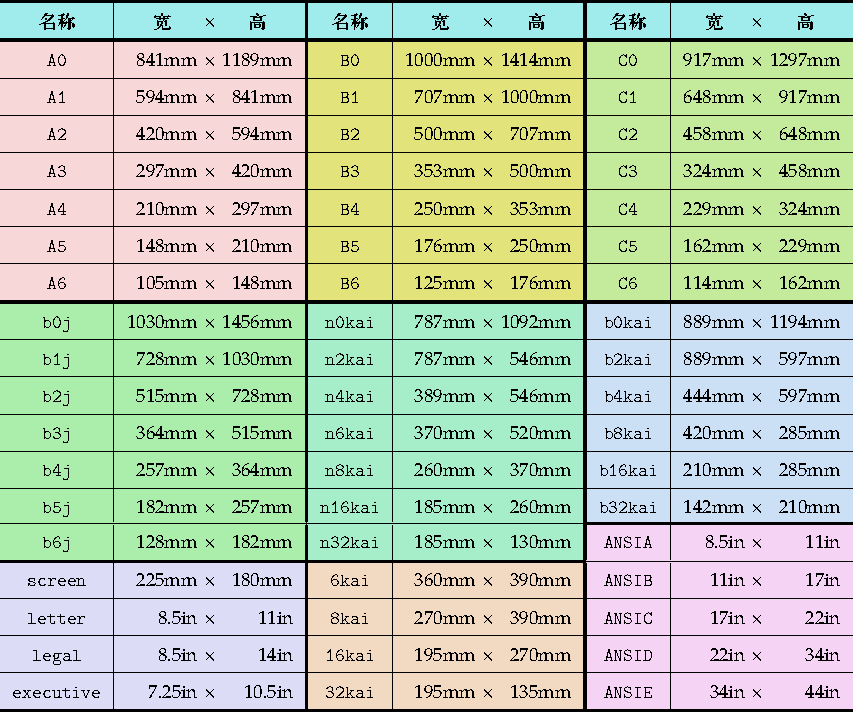
\includegraphics{cus-aux/tab-defined-papername}}
  \caption{预定义的纸张名}\label{tab:defined-papername}
\end{table}

\begin{keyval}[path=layout]{paperorientation,orientation,landscape,portrait,direction}
  \begin{syntax}
    paperorientation|orientation = <&landscape|portrait>
    landscape &&
    portrait  &&
    direction = <&bigwidth|bigheight|normal|inverse>
  \end{syntax}
设置纸张方向。使用 \opt{portrait} 时,纸张高度大于宽度。\opt{landscape} 则反之。

\opt{direction} 的 \opt{bigheight} 和 \opt{normal} 相当于 \opt{portrait},
\opt{bigwidth} 和 \opt{inverse} 相当于 \opt{landscape}。

使用 \opt{papername} 等选项时,将自动设置纸张方向,使得实际纸张宽高与所给一致。
\end{keyval}

\begin{keyval}[path=layout]{layout,layoutname,
  layoutwidth,layoutheight,layoutsize,
  layouthoffset,layoutvoffset,layoutoffset}
设置 \gpart{layout} 部分大小。

见 \pkgdoc{geometry}。
\end{keyval}

\subsection{主体尺寸}

此小节与 \pkg{geometry} 对应部分的用法和作用相同。

\begin{keyval}[path=layout]{hscale,vscale,scale}
  \begin{syntax}
    hscale = \marg{正实数} & 0.7
    vscale = \marg{正实数} & 0.7
    scale  = \{\meta{hscale},\meta{vscale}\} 或 \marg{正实数}
  \end{syntax}
设置 \gpart{total part} 部分的宽高与 纸张宽高的比率。
\end{keyval}

\begin{keyval}[path=layout]{totalwidth,width,totalheight,height,total}
  \begin{syntax}
    totalwidth |width  = \marg{长度}
    totalheight|height = \marg{长度}
    total              = \{\meta{totalwidth},\meta{totalheight}\} 或 \marg{长度}
  \end{syntax}
设置 \gpart{total part} 部分的宽高。
\end{keyval}

\begin{keyval}[path=layout]{textwidth,textheight,body,text}
  \begin{syntax}
    textwidth  = \marg{长度}
    textheight = \marg{长度}
    body       = \{\meta{textwidth},\meta{textheight}\}
    text       = \marg{长度}
  \end{syntax}
设置 \tn{textwidth}、\tn{textheight},即 \gpart{body} 部分的宽高。
\end{keyval}

\begin{keyval}[path=layout]{lines}
  \begin{syntax}
    lines = \marg{行数}
  \end{syntax}
根据 \meta{行数} 设置 \opt{textheight}。\meta{行数} 一般为正整数。
\end{keyval}

\begin{keyval}[path=layout]{includehead,includefoot,
  includeheadfoot,includehf}
  \begin{syntax}
    includehead = <&\TTF> & false 
    includefoot = <&\TTF> & false
    includeheadfoot|includehf = <&\TTF>
  \end{syntax}
控制是否将页眉(\tn{headheight}、\tn{headsep})、页脚(\tn{footskip})
计入 \gpart{total part} 部分中。
\end{keyval}

\begin{keyval}[path=layout]{includemarginpar,includemp}
  \begin{syntax}
    includemarginpar|includemp = <&\TTF> & false 
  \end{syntax}
控制是否将旁注(\tn{marginparwidth}、\tn{marginparsep})计入 \gpart{body} 部分中。
\end{keyval}

\begin{keyval}[path=layout]{includeall}
  \begin{syntax}
    includeall = <&\TTF> & false 
  \end{syntax}
设置 \opt{includeheadfoot} 及 \opt{includemarginpar}。
\end{keyval}

\begin{keyval}[path=layout]{ignorehead,ignorefoot,
  ignoreheadfoot,ignorehf}
  \begin{syntax}
    ignorehead = <&\TTF> & false 
    ignorefoot = <&\TTF> & false
    ignoreheadfoot|ignorehf = <&\TTF>
  \end{syntax}
在计算垂直方向的尺寸时,不考虑页眉、页脚。但不修改页眉页脚的尺寸。
\end{keyval}

\begin{keyval}[path=layout]{ignoremarginpar,ignoremp}
  \begin{syntax}
    ignoremarginpar|ignoremp = <&\TTF> & false 
  \end{syntax}
在计算水平方向的尺寸时,不考虑旁注的尺寸。但不修改旁注的尺寸。
\end{keyval}

\begin{keyval}[path=layout]{ignoreall}
  \begin{syntax}
    ignoreall = <&\TTF> & false 
  \end{syntax}
设置 \opt{ignoreheadfoot} 及 \opt{ignoremarginpar}。
\end{keyval}

\begin{keyval}[path=layout]{heightrounded}
  \begin{syntax}
    heightrounded = <&\TTF> & false
  \end{syntax}
如果设置为真,则将 \opt{textheight} 设置为不小于原 \opt{textheight} 且满足关系:
\[ n\times{}\text{\tn{baselineskip}}{}+{}\text{\tn{topskip}}\] 
的最小值。
\end{keyval}

% from geometry.dtx
\thisfloatsetup{margins=hangoutside,capposition=beside,
  capbesideposition={top,outside},floatwidth=\textwidth}
\begin{figure}[htb]
 \centering\small
 {\unitlength=.65pt
 \begin{picture}(460,525)(0,0)
 \put( 20,310){\framebox(120,170){}}
 \put( 20,507){\makebox(120,0)[bl]%
 {\textbf{(a)}~\opt{includeheadfoot}}}
 \put( 20,460){\line(1,0){120}}\put( 20,450){\line(1,0){120}}
 \put( 20,330){\line(1,0){120}}
 \put( 20,485){\makebox(120,0)[br]{\gpart{total body}}}
 \put( 20,335){\makebox(120,0)[bc]{\texttt{textwidth}}}
 \put(150,470){\makebox(0,0)[l]{\texttt{headheight}}}
 \put(150,450){\makebox(0,0)[l]{\texttt{headsep}}}
 \put(150,390){\makebox(0,0)[l]{\texttt{textheight}}}
 \put(150,320){\makebox(0,0)[l]{\texttt{footskip}}}
 \put( 10,460){\makebox(120,20)[bc]{\gpart{head}}}
 \put( 10,320){\makebox(120,140)[c]{\gpart{body}}}
 \put( 10,310){\makebox(120,10)[c]{\gpart{foot}}}
 \put(250,310){\framebox(120,170){}}
 \put(250,507){\makebox(120,0)[bl]%
 {\textbf{(b)}~\opt{includeall}}}
 \put(250,460){\line(1,0){95}}\put(250,450){\line(1,0){95}}
 \put(250,330){\line(1,0){95}}\put(345,330){\line(0,1){120}}
 \put(350,330){\line(0,1){120}}\put(350,450){\line(1,0){20}}
 \put(350,330){\line(1,0){20}}
 \put(250,485){\makebox(120,0)[br]{\gpart{total body}}}
 \put(250,460){\makebox(95,20)[bc]{\gpart{head}}}
 \put(250,320){\makebox(95,140)[c]{\gpart{body}}}
 \put(385,390){\makebox(95,0)[cl]%
 {\gpart{\shortstack[l]{marginal\\note}}}}
 \put(250,310){\makebox(95,10)[c]{\gpart{foot}}}
 \put(250,335){\makebox(95,0)[bc]{\texttt{textwidth}}}
 \multiput(360, 390)(4,0){6}{\line(1,0){2}}
 \multiput(348,333)(0,-4){12}{\line(0,1){2}}
 \multiput(360,333)(0,-4){8}{\line(0,1){2}}
 \put(355,292){\makebox(0,0)[bl]{\texttt{marginparwidth}}}
 \put(345,275){\makebox(0,0)[bl]{\texttt{marginparsep}}}
 \put( 20, 40){\framebox(120,170){}}
 \put( 20,237){\makebox(120,0)[bl]%
 {\textbf{(c)}~\opt{includefoot}}}
 \put( 20, 60){\line(1,0){120}}
 \put( 20,215){\makebox(120,0)[br]{\gpart{total body}}}
 \put(150,130){\makebox(0,0)[l]{\texttt{textheight}}}
 \put(150, 50){\makebox(0,0)[l]{\texttt{footskip}}}
 \put( 20, 50){\makebox(120,160)[c]{\gpart{body}}}
 \put( 20, 40){\makebox(120,10)[c]{\gpart{foot}}}
 \put( 20, 65){\makebox(120,10)[c]{\texttt{textwidth}}}
 \put(250, 40){\framebox(120,170){}}
 \put(250,237){\makebox(120,0)[bl]%
 {\textbf{(d)}~\opt{includefoot}, \opt{includemp}}}
 \put(250, 60){\line(1,0){95}}\put(350, 60){\line(1,0){20}}
 \put(250,215){\makebox(120,0)[br]{\gpart{total body}}}
 \put(250, 50){\makebox(95,160)[c]{\gpart{body}}}
 \put(385,130){\makebox(95,0)[cl]%
 {\gpart{\shortstack[l]{marginal\\note}}}}
 \put(250, 40){\makebox(95,10)[c]{\gpart{foot}}}
 \put(250, 65){\makebox(95,0)[bc]{\texttt{textwidth}}}
 \put(345, 60){\line(0,1){150}}\put(350, 60){\line(0,1){150}}
 \multiput(360, 130)(4,0){6}{\line(1,0){2}}
 \multiput(348, 63)(0,-4){12}{\line(0,1){2}}
 \multiput(360, 63)(0,-4){8}{\line(0,1){2}}
 \put(355,22){\makebox(0,0)[bl]{\texttt{marginparwidth}}}
 \put(345, 5){\makebox(0,0)[bl]{\texttt{marginparsep}}}
 \end{picture}}
 \captionsetup{labelsep=newline}
 \caption[不同模式下的 total part]{\small
 \ifLabelOdd{fig:geometry-modes}{\raggedright}{\raggedleft}%
  不同模式下的 \gpart{total body}。
  (a) \opt{includeheadfoot},(b) \opt{includeall},(c) \opt{includefoot}
  及 (d) \opt{includefoot},\opt{includemp}。
  如果 \opt{reversemarginpar} 设置为真,则交换 \gpart{marginal note} 与 \gpart{body}
  的位置。如果设置了 \opt{twoside},则依据奇偶页交换 \gpart{marginal note}。}
 \label{fig:geometry-modes}
\end{figure}

\begin{keyval}[path=layout]{hdivide,vdivide,divide}
  \begin{syntax}
    hdivide = \{\meta{left margin},\meta{width},\meta{right margin}\}
    vdivide = \{\meta{top margin},\meta{height},\meta{bottom margin}\}
    divide  = \{\meta{length_1},\meta{length_2},\meta{length_3}\}
  \end{syntax}
设置两个值,将另一个留空或 \verb|*|。
\end{keyval}


\subsection{边距}

\nofuncskip
\begin{keyval}[path=layout]{leftmargin,left,lmargin,inner,
  rightmargin,right,rmargin,outer,hmargin,horizontalmargin}
  \begin{syntax}
    lmargin|leftmargin |left |inner = \marg{内侧边距}
    rmargin|rightmargin|right|outer = \marg{外侧边距}
    hmargin|horizontalmargin  = \{\meta{inner},\meta{outer}\} 或 \marg{水平边距}
  \end{syntax}
设置内外侧边距。注意,不论是否使用 \opt{twoside},它们的含义都是相同的。
\end{keyval}

\begin{keyval}[path=layout]{topmargin,top,tmargin,bottommargin,bottom,bmargin,verticalmargin}
  \begin{syntax}
    tmargin|topmargin   |top    = \marg{顶部边距}
    bmargin|bottommargin|bottom = \marg{底部边距}
    vmargin|verticalmargin      = \{\meta{top},\meta{bottom}\} 或 \marg{垂直边距}
  \end{syntax}
设置上下边距。
\end{keyval}

\begin{keyval}[path=layout]{horizontalmarginratio,hmarginratio,
  verticalmarginratio,vmarginratio,marginratio}
  \begin{syntax}
    hmarginratio|horizontalmarginratio = \marg{inner ration}:\marg{outer ratio}
    vmarginratio|verticalmarginratio   = \marg{top ratio}:\marg{bottom ratio} & 2:3
    marginratio = \{\meta{hmargin ratio},\meta{vmargin ratio}\} 或 \marg{margin ratio}
  \end{syntax}
设置内外边距、上下边距的比率。

使用 \opt{oneside} 时 \opt{hmarginratio} 初始为 \texttt{1:1},
使用 \opt{twoside} 时 \opt{hmarginratio} 初始为 \texttt{2:3}。
\end{keyval}

\begin{keyval}[path=layout]{hcentering,vcentering,centering}
  \begin{syntax}
    hcentering = <&\TTF> 
    vcentering = <&\TTF> & false 
    centering  = <&\TTF>
  \end{syntax}
设置 \opt{hmarginratio}、\opt{vmarginratio} 为 \texttt{1:1}。
\end{keyval}

\begin{keyval}[path=layout]{twoside,asymmetric,reversemarginpar,reversemp}
  \begin{syntax}
    twoside &&
    asymmetric &&
    reversemarginpar|reversemp = <&\TTF> & false 
  \end{syntax}
设置左右边距根据奇偶页进行切换。\opt{asymmetric} 并不实际切换,而是修改长度,见 \pkgdoc{geometry}。
\end{keyval}

\begin{keyval}[path=layout]{bindingoffset}
  \begin{syntax}
    bindingoffset = \marg{长度}
  \end{syntax}
从内侧移除 \meta{长度}。
\end{keyval}

% from geometry.dtx
\thisfloatsetup{margins=hangoutside,capposition=beside,
  capbesideposition={top,outside},floatwidth=\textwidth}
\begin{figure}[htb]
 \centering\small
 {\unitlength=.65pt
 \begin{picture}(500,270)(0,0)
 \put(20,0){\framebox(170,230){}}
 \put(20,255){\makebox(80,20)[l]{\textbf{a)}~every page for oneside or}}
 \put(20,240){\makebox(80,20)[l]{\hspace{3ex}odd pages for twoside}}
 \put(110,225){\makebox(80,20)[r]{\gpart{paper}}}
 \put(55,37){\framebox(110,170)[tc]{\gpart{total body}}}
 \multiput(38,0)(0,7){33}{\line(0,1){4}}
 \put(38,100){\vector(1,0){17}}\put(55,100){\vector(-1,0){17}}
 \put(60,95){\makebox(80,10)[l]{\texttt{left}}}
 \put(60,80){\makebox(80,10)[l]{(\texttt{inner})}}
 \put(165,100){\vector(1,0){25}}\put(190,100){\vector(-1,0){25}}
 \put(195,95){\makebox(80,10)[l]{\texttt{right}}}
 \put(195,80){\makebox(80,10)[l]{(\texttt{outer})}}
 \put(20,16){\vector(1,0){18}}
 \put(45,10){\makebox(80,10)[bl]{\texttt{bindingoffset}}}
 \put(280,255){\makebox(80,20)[l]{\textbf{b)}~even (back) pages for twoside}}
 \put(280,0){\framebox(170,230){}}
 \put(370,225){\makebox(80,20)[r]{\gpart{paper}}}
 \put(305,37){\framebox(110,170)[tc]{\gpart{total body}}}
 \multiput(432,0)(0,7){33}{\line(0,1){4}}
 \put(280,100){\vector(1,0){25}}\put(305,100){\vector(-1,0){25}}
 \put(310,95){\makebox(80,10)[l]{\texttt{outer}}}
 \put(310,80){\makebox(80,10)[l]{(\texttt{right})}}
 \put(415,100){\vector(1,0){17}}\put(432,100){\vector(-1,0){17}}
 \put(373,95){\makebox(80,10)[l]{\texttt{inner}}}
 \put(373,80){\makebox(80,10)[l]{(\texttt{left})}}
 \put(450,16){\vector(-1,0){18}}
 \put(330,10){\makebox(80,10)[bl]{\texttt{bindingoffset}}}
 \end{picture}}
 \captionsetup{labelsep=newline}
 \caption[\texttt{bindingoffset} 选项]{%
  \raggedleft\small
  The option \opt{bindingoffset} adds the specified length to the inner margin.
  Note that \opt{twoside} option swaps the horizontal margins and the
  marginal notes together with \opt{bindingoffset} on even pages (see
  \textbf{b}), but \opt{asymmetric} option suppresses the swap of the
  margins and marginal notes (but \opt{bindingoffset} is still swapped).}
 \label{fig:bindingoffset}
\end{figure}


\subsection{原有长度}

本小节描述几个 \LaTeXe 原有的长度变量。

\begin{keyval}[path=layout]{footnotesep}
  \begin{syntax}
    footnotesep = \marg{弹性长度}
  \end{syntax}
设置 \tn{skip}\tn{footins},即正文底部与脚注顶部的距离。
\end{keyval}

\begin{keyval}[path=layout]{marginparwidth,marginpar,marginparsep,nomarginpar,nomp}
  \begin{syntax}
    marginparwidth|marginpar = \marg{长度}
    marginparsep = \marg{长度}
    nomarginpar|nomp &&
  \end{syntax}
设置旁注宽度及旁注与正文的距离。\opt{nomarginpar} 将它们设置为 \texttt{0pt}。
\end{keyval}

\begin{keyval}[path=layout]{columnsep,twocolumn,onecolumn}
  \begin{syntax}
    columnsep = \marg{长度}
    twocolumn &&
    onecolumn &&
  \end{syntax}
设置 \tn{columnsep},即两栏之间的距离。
\end{keyval}

\begin{keyval}[path=layout]{hoffset,voffset,offset}
  \begin{syntax}
    hoffset = \marg{长度}
    voffset = \marg{长度}
    offset  = \{\meta{hoffset},\meta{voffset}\} 或 \marg{长度}
  \end{syntax}
设置 \tn{hoffset}、\tn{voffset}。
\end{keyval}


\subsection{页眉页脚}\label{sec:geometry-headfoot}

\nofuncskip 
\begin{keyval}[path=layout]{headheight,head,headsep}
  \begin{syntax}
    head|headheight = \marg{长度}
    headsep = \marg{长度}
    nohead
  \end{syntax}
\opt{headheight} 设置 \tn{headheight},即页眉的高度。

\opt{headsep} 设置 \tn{headsep},即页眉与正文之间的距离。

\opt{nohead} 将它们设置为 \texttt{0pt}。
\end{keyval}

\begin{keyval}[path=layout]{footskip,foot,nofoot}
  \begin{syntax}
    footskip|foot = \marg{弹性长度}
  \end{syntax}
设置 \tn{footskip},即正文最后一行的基线与页脚基线的距离。

\opt{nofoot} 将它设置为 \texttt{0pt}。
\end{keyval}

\begin{keyval}[path=layout]{noheadfoot,nohf}
  \begin{syntax}
    noheadfoot|nohf &&
  \end{syntax}
同时设置 \opt{nohead} 和 \opt{nofoot}
\end{keyval}

\begin{keyval}[path=layout]{headoffset,footoffset,hfoffset}
  \begin{syntax}
    headoffset = \marg{长度} & 0pt 
    headoffset = \oarg{位置} \marg{长度}
  \end{syntax}
设置页眉页脚偏移量。

\meta{位置} 为 \texttt{O}、\texttt{E} 与 \texttt{L}、\texttt{C}、\texttt{R} 的组合。
这五个值分别代表奇偶、左中右。不区分大小写。

若 \meta{长度} 为正值,则相较于 \opt{textwidth} 伸长 \meta{长度}。否则,缩短 \meta{长度}。

此选项在直排文档中可能无效。
\end{keyval}

\subsection{杂项}

本小节列出其它几个选项。未列出的选项请参考 \pkgdoc{geometry}。

% \nofuncskip
\begin{keyval}[path=layout]{showframe,showmarking,marking}
  \begin{syntax}
    showframe = <&\TTF> & false 
    showcrop  = <&\TTF> & false 
    showmarking|marking = <&\TTF> & false 
  \end{syntax}
\opt{showframe} 显示各部分的外框。\opt{showcrop} 在 \gpart{layout} 四角显示裁剪标记。
\opt{marking} 在各部分着以彩色背景。
\end{keyval}

\begin{keyval}[path=layout]{preset,name}
  \begin{syntax}
    preset|name = \marg{preset name}
  \end{syntax}
使用预设值 \meta{preset name}。
\end{keyval}

% \begin{keyval}[path=layout]{verbose}
%   \begin{syntax}
%     verbose = <&\TTF> & false 
%   \end{syntax}
% 将各变量的结果显示在终端中。设置为 \opt{false} 时,仍将其写入日志文件中。

% 仅可用于导言区。
% \end{keyval}

% \begin{keyval}[path=layout]{pass}
%   \begin{syntax}
%     pass &&
%   \end{syntax}
% 仅可用于导言区。
% \end{keyval}


\subsection{设置页眉页脚}\label{sec:pagestyle}

本小节设置页眉页脚内容的接口。关于设置页眉页脚位置和高度的接口,见\cref{sec:geometry-headfoot}。

本节所述内容可能在直排文档中不可用。

本节所述的功能主要通过 \pkg{fancyhdr} 实现。

\begin{function}{\usepagestyle}
  \begin{syntax}
    \verb|\usepagestyle| \marg{pagestyle}
  \end{syntax}
使用页眉页脚的样式 \meta{pagestyle}。

有一个预定义的样式 \texttt{totalempty},它将页眉页脚设置为空,并将页眉页脚横线的厚度设为 \texttt{0pt}。
\end{function}

\begin{function}{\setpagestyle}
  \begin{syntax}
    \verb|\setpagestyle|   \marg{pagestyle} \marg{code}
    \verb|\setpagestyle|   \marg{pagestyle_1} \oarg{pagestyle_2} \marg{code}
    \verb|\setpagestyle| * \marg{pagestyle_1} \oarg{pagestyle_2} \marg{code}
  \end{syntax}
设置样式 \marg{pagestyle},或基于样式 \meta{pagestyle_2} 设置 \meta{pagestyle_1}。

带 \verb|*| 的,仅设置而不使用。不带 \verb|*| 的,还会立刻使用该样式。
\end{function}

\begin{function}{\sethead,\setfoot,\setheadfoot,
  \setlefthead,\setcenterhead,\setrighthead,
  \setleftfoot,\setcenterfoot,\setrightfoot}
  \begin{syntax}
    \verb|\sethead|         \,\marg{code}
    \verb|\sethead| \oarg{位置} \marg{code}
    \verb|\setcenterhead|           \,\marg{奇偶页}
    \verb|\setcenterhead| \oarg{偶数页} \marg{奇数页}
  \end{syntax}
设置页眉页脚的内容。

\meta{位置} 为 \texttt{O}、\texttt{E}, \texttt{L}、\texttt{C}、\texttt{R},\texttt{H}、\texttt{F} 此三类的组合。
这七个个值分别代表奇偶、左中右、页眉页脚。不区分大小写。

如某一类未给出,则视为该类的全部值都给出。但 \cs{sethead}、\cs{setfoot} 分别为 \texttt{H}、\texttt{F}。

例如,在 \cs{sethead} 中,\verb|L| 代表 \verb|OLF,ELF|。

它们可以直接用在导言区和正文中,将修改本页及其后页面的页眉页脚。但最好用于 
\cs{setpagestyle} 命令中,统一设置页眉页脚。
\end{function}

\begin{function}{\setheadrulewidth,\setfootrulewidth}
  \begin{syntax}
    \verb|\setheadrulewidth| \marg{长度表达式}
  \end{syntax}
设置页眉、页脚横线的厚度。

(即宏 \tn{headrulewidth}、\tn{footrulewidth} 的值。)
\end{function}

\begin{function}{\setheadruleskip,\setfootruleskip}
  \begin{syntax}
    \verb|\setheadruleskip| \marg{skip expr}
  \end{syntax}
设置页眉、页脚横线与页眉、页脚文字的距离。

(即宏 \tn{headruleskip}、\tn{footruleskip} 的值。)
\end{function}

\begin{function}{\setheadrule,\setfootrule}
  \begin{syntax}
    \verb|\setheadrule| \marg{code}
  \end{syntax}
设置页眉、页脚的横线。页眉的横线的总高度最好为 0。
\end{function}

\begin{function}{\setheadinit,\setfootinit,\setheadfootinit}
  \begin{syntax}
    \verb|\setheadinit| \marg{code}
  \end{syntax}
在输出页眉页脚前要执行的 \meta{code}。
\end{function}

\begin{function}{\fancycenter}
  \begin{syntax}
    \verb|\fancycenter| \marg{left} \marg{center} \marg{right}
    \verb|\fancycenter| \oarg{distance} \oarg{stretch} \marg{left} \marg{center} \marg{right}
  \end{syntax}
它创建一个盒子,使得 \meta{center} 位于当前行(或盒子)的中心。可以用于正文中。

\meta{center} 的中心与 \meta{left}、\meta{right} 的中心的距离可能并不一致。
\end{function}

\begin{xample}
\fancycenter{L}{CCCC}{RRRRRRRRRRRRRRRR}
\stopxamplecode
\xampleprint
\end{xample}

\begin{function}[EXP]{\iftopfloat,\ifbotfloat,\iffloatpage,\iffootnote}
  \begin{syntax}
    \verb|\iftopfloat| \marg{true} \marg{false}
  \end{syntax}
检测当前页是否顶部、底部有浮动体,或当前页是否是浮动体页,或当前页是否有脚注。
\end{function}


\section{盒子和填充,\texorpdfstring{\cusmodule{box}}{box}模块}

\cusmodule{box} 用于提供盒子构造、内容填充等内容。


\subsection{Framed}

\cusmodule{box} 模块定义了一个简易的可跨页的盒子环境 \env{Framed},相较于 
\pkg{tcolorbox} 宏包提供的环境来说,使用此环境的速度更快。它也可配合 \pkg{tcolorbox}
宏包使用。

\begin{function}[type=environment]{Framed}
  \begin{syntax}
    \verb|\begin{Framed}| \oarg{frame key-val}
    ~~... 
    \verb|\end{Framed}|
  \end{syntax}
创建一个可跨页的盒子。若在另一个盒子内则不可跨页。
\end{function}

\begin{keyval}[path=frame]{outer-sep}
  \begin{syntax}
    outer-sep = \marg{skip expr} & 8pt plus 8pt minus 6pt 
  \end{syntax}
设置盒子与上下文的间距。
\end{keyval}

\begin{keyval}[path=frame]{sep}
  \begin{syntax}
    sep = \marg{长度表达式} & \V{3\fboxsep}
  \end{syntax}
设置变量 \tn{cusframesep},即盒子外框与内容的间距。
\end{keyval}

\begin{keyval}[path=frame]{rule-width}
  \begin{syntax}
    rule-width = \marg{长度表达式} & \V\fboxrule
  \end{syntax}
设置变量 \tn{cusframerule},即盒子外框的厚度。
\end{keyval}

\begin{keyval}[path=frame]{frame,frame*,
  first,first*,middle,middle*,last,last*,
  whole,whole*}
  \begin{syntax}
    frame  = \marg{code}
    frame* = \marg{code width 1 parameter}
  \end{syntax}
\opt{frame} 设置盒子外框。

\opt{first},\opt{middle},\opt{last} 设置分页盒子的前、中、后三部分的外框。

\opt{whole} 设置未分页盒子的外框。

\meta{code} 其后可接一个参数,这个参数为分页后的盒子。
\meta{code with 1 parameter} 显式给出变量 \verb|#1|。
\end{keyval}

\begin{keyval}[path=frame]{init}
  \begin{syntax}
    init = \marg{code}
  \end{syntax}
盒子中执行的初始化代码。
\end{keyval}

\begin{keyval}[path=frame]{width,ratio}
  \begin{syntax}
    width = \marg{长度表达式} & \V\textwidth
    ratio = \marg{数值表达式} & 1
  \end{syntax}
\opt{ratio} 设置盒子内容(含边框)占 \opt{width} 的比率。
\end{keyval}

\begin{keyval}[path=frame]{align,
  left,center,right,inner,outer}
  % absinner,absouter,inner*,outer*,
  \begin{syntax}
    align = <&left|center|right|inner|outer> & center 
  \end{syntax}
设置水平对齐方式。当 $ 0 <{} \text{\meta{ratio}} {}< 1 $ 时才有效。
\end{keyval}

\begin{xample}
\begin{Framed}[ratio=.8,center,
  rule-width=2pt,
  frame={\setlength{\fboxsep}{\cusframesep}%
          \setlength{\fboxrule}{\cusframerule}%
          \fcolorbox{purple}{cyan!50}}]
\zhlipsum[9][name=zhufu]
\end{Framed}
\stopxamplecode
\xampleprint 
\vskip 1pt 
\end{xample}

\begin{keyval}[path=frame]{ignore-warnings}
  \begin{syntax}
    ignore-warnings &&
  \end{syntax}
忽略部分警告。
\end{keyval}


\subsection{Filler}

“filler”是用以填充空间的那部分内容。如 \LaTeXe 的 \tn{hrulefill} 是用水平直线填充,
\tn{dotfill} 是用句点填充,\tn{hspace} 是用空白填充。

\cusmodule{box} 提供了几个创建 filler 的命令。

\begin{function}{\dashfiller}
  \begin{syntax}
    \verb|\dashfiller|
    \verb|\dashfiller| \marg{filler width}
    \verb|\dashfiller| \oarg{raise}\oarg{sep width}\oarg{rule width}
    \verb|\dashfiller| \oarg{raise} \marg{filler width}\oarg{sep width}\oarg{rule width}
  \end{syntax}
使用虚线填充,虚线宽和虚线间的距离近似为 \meta{sep width},使得虚线充满 \meta{filler width}。

\begin{itemize}[nosep]
  \item \meta{filler width} 为总宽度,默认值为 \tn{linewidth}。
  \item \meta{raise} 为虚线升高的高度,默认为 \texttt{0pt}。
  \item \meta{sep width} 为虚线宽和虚线间的距离,默认为 \texttt{1ex}。
  \item \meta{rule width} 为虚线的厚度,默认为 \texttt{0.4pt}。
\end{itemize}
\end{function}

\begin{xample}
\noindent\llap{|}\dashfiller \par % 总长为 \linewidth 
\noindent\llap{|}\dashfiller [.5ex] \par % 升高 .5ex
% 升高 .5ex,宽 3pt,注意第二个可选参数前不能有空格
\noindent\llap{|}\dashfiller [.5ex][3pt] \par 
\stopxamplecode
\xampleprint 
\end{xample}

\begin{function}{\filler}
  \begin{syntax}
    \verb|\filler| \oarg{filler key-val}
  \end{syntax}
使用给定内容填充。
\end{function}

\begin{keyval}[path=filler]{size,size*}
  \begin{syntax}
    size  = \marg{skip expr}
    size* = \marg{长度}
  \end{syntax}
设置填充的长度。\opt{size*} 填充的长度是弹性的。

注意在行间数学模式中(\env{equation}、\env{align} 等环境)弹性的那部分长度无效。
\end{keyval}

\begin{keyval}[path=filler]{space,hspace,hspace*,vspace,vspace*,not-space}
  \begin{syntax}
    space   = \marg{code}
    hspace  = \marg{skip expr}
    hspace* = \marg{skip expr}
    vspace  = \marg{skip expr}
    vspace* = \marg{skip expr}
    not-space &&
  \end{syntax}
使用空白填充。使用它后,其它选项无效。

\meta{code} 是填充的内容,如 \verb|\hspace{1cm}|,\verb|\vspace*{1cm}|。

\opt{hspace} 相当于设置 \verb|space=\hspace|\marg{skip expr}。

\opt{hspace*} 相当于设置 \verb|space=\hspace*|\marg{skip expr}。

\opt{vspace} 相当于设置 \verb|space=\vspace|\marg{skip expr}。

\opt{vspace*} 相当于设置 \verb|space=\vspace*|\marg{skip expr}。

由于用 space 填充的优先级最高,若设置使用 space 填充后,要使用其它类型来填充,需使用
\opt{not-space} 或将 \opt{space} 设置为空。若后续仍设置了 \opt{space},则仍会使用 space 填充。
\end{keyval}

\begin{xample}
左 \fbox{\strut \filler [hspace=5cm]} 右间隔约 5cm。

左 \filler[space] 右拉开。

左 \filler[space] 中 \filler[space] 右拉开。
\stopxamplecode
\xampleprint
\end{xample}

\begin{keyval}[path=filler]{color}
  \begin{syntax}
    color = <{color expr}>
  \end{syntax}
设置颜色 \texttt{cusfiller},即填充的颜色。
\end{keyval}

\begin{keyval}[path=filler]{content,box,box*,clear-box}
  \begin{syntax}
    content = <{content}>
    box     = <{content}>
    box*    = <{长度表达式}> <{content}>
    clear-content &&
    clear-box &&
    not-content &&
  \end{syntax}
使用长 \meta{长度表达式} 的 \meta{content} 填充。

\opt{content} 和 \opt{box} 选项基本一致,只是 \opt{content} 会自动设置颜色,而
\opt{box} 则需使用 \tn{color} 或 \cs{color_select:n} 来设置颜色。

使用 \opt{content} 将使用 \meta{content} 的自然宽度,而 \opt{box*} 则使用指定的宽度。

当设置了 \opt{box} 或 \opt{box*} 后,\opt{content} 无效,除非使用 \opt{clear-box} 清除 box。
\end{keyval}

\begin{keyval}[path=filler]{dash,sep,rule,raise,full,is-dash}
  \begin{syntax}
    dash|sep = \marg{dash length} & 0pt 
    rule     = \marg{rule width} & 0.4pt 
    raise    = \marg{raise height} & 0pt 
    full     = <&\TTF> & false 
    is-dash &&
  \end{syntax}
使用虚线填充。

虚线宽和虚线间距为 \meta{dash length},厚度为 \meta{rule width},升高 \meta{raise height}。

若 \meta{dash length} 为 \texttt{0pt},则使用实线填充。

如果设置 \opt{full} 为真,则相当于 \cs{dashfiller}。
\end{keyval}

\begin{keyval}[path=filler]{solid,dashed,dotted,cdotted}
  \begin{syntax}
    solid &&
    dashed  = \marg{长度}
    dotted  = \marg{间距}
    cdotted = \marg{间距}
  \end{syntax}
使用实线、虚线、句点或 \tn{cdot} 填充。
\end{keyval}

\begin{xample}
\def\BL{\noindent\llap{|}}%
\BL \filler[color=red, solid, rule=2pt] \par
\BL \filler[color=red, dashed, rule=0.5ex] \par 
\BL \filler[color=red, dashed, rule=0.5ex, full] \par 
\BL \filler[color=red, dotted] \par 
\BL \filler[color=red, cdotted] \par 
\BL \filler[color=red, cdotted=1cm, align] \par % 每个点都是对齐的
\BL \filler[color=red, cdotted=1cm, center] \par % 每个点的间距都是 1cm
\BL \filler[color=red, cdotted=1cm, spread] % 每个点的间距都相等,可能超过1cm
\stopxamplecode
\xampleprint
\end{xample}

\begin{keyval}[path=filler]{type,align,center,spread}
  \begin{syntax}
    type  = <&align|center|spread> & align 
    align &&
    center &&
    spread &&
  \end{syntax}
构造填充的方式。

\begin{itemize}[nosep]
  \item \opt{align}:每个同种 filler 都是无限长的对齐的填充中的一部分,因此,它们处处都是对齐的;
  \item \opt{center}:把用以填充的盒子紧挨着排列,两头留下相等的空白;
  \item \opt{spread}:把多余的空白均匀地分布在盒子中间及两侧。
\end{itemize}
\end{keyval}

\begin{texnote}
实际这三种方式分别对应 \tn{leaders}、\tn{cleaders}、\tn{xleaders}。
\end{texnote}

\begin{function}{\atleastfiller}
  \begin{syntax}
    \verb|\atleastfiller| \marg{dim expr}
    \verb|\atleastfiller| \oarg{filler key-val} \marg{dim expr}
  \end{syntax}
填充的长度至少为 \meta{dim epxr},太短的将自动断行。
\end{function}

\begin{xample}
我能吞下玻璃而不伤身体,I can eat glass, it dosen't hurt me.%
\atleastfiller[cdotted=1em]{5cm}断行。

我能吞下玻璃而不伤身体。\atleastfiller[cdotted=1em]{5cm}不断。
\stopxamplecode
\xampleprint 
\end{xample}

\begin{function}{\breakablefiller}
  \begin{syntax}
    \verb|\breakablefiller|
    \verb|\breakablefiller| \oarg{filler key-val}
  \end{syntax}
可自动断行的 filler。
\end{function}

\begin{xample}
\framebox[3cm]{可断} \breakablefiller[cdotted=1em] \framebox[3cm]{模式。}

\framebox[7cm]{可断} \breakablefiller[cdotted=1em] \framebox[7cm]{模式。}
\stopxamplecode
\xampleprint
\end{xample}

下例展示了制作多行填充的例子。
\begin{xample}
\newcommand\filllines[4][]{{% filler key-val, before, lines, after
  #2\filler[#1]%
  \Replicate{#3-1}{\break \rule{0pt}{0.7\baselineskip}\filler[#1]}%
  #4\par}}

我能吞下玻璃而不伤身体,I can eat glass, it dosen't hurt me.
\filllines{\linespread{2}\selectfont}{3}{。\hspace*{1em}}

我能吞下玻璃而不伤身体,I can eat glass, it dosen't hurt me.
\filllines[color=red,dotted]{\linespread{2}\selectfont}{3}{。\hspace*{1em}}

% 整行
\filllines [raise=-.5ex]{\linespread{2}\selectfont \noindent\strut}{3}{ 整行。\hspace*{1em}}
\stopxamplecode
\xampleprint  
\end{xample}


\subsection{多栏文字}

\CusTeX 中排版多栏文字有两种方式,本节描述其中一种,使用 \pkg{multicol} 宏包实现。

关于每个内部变量的详细用法,可以参考 \pkgdoc{multicol}。

\begin{function}{\startmulticolumns,\stopmulticolumns}
  \begin{syntax}
    \verb|\startmulticolumns| \oarg{multicolumns key-val}
    ~~<content>
    \verb|\stopmulticolumns|
  \end{syntax}
将 \meta{content} 以多栏排版。
\end{function}

\begin{keyval}[path=multicolumns]{columns,cols}
  \begin{syntax}
    columns|cols = \marg{整数表达式} & 2
  \end{syntax}
设置多栏数。也可不必写出键名,只写数字。可用的栏数为 1--20。
\end{keyval}

\begin{keyval}[path=multicolumns]{outer-sep}
  \begin{syntax}
    outer-sep = \marg{skip expr} & 12.0pt plus 4.0pt minus 3.0pt
  \end{syntax}
设置 \tn{multicolsep},即多栏文字与上下文的间距。
\end{keyval}

\begin{keyval}[path=multicolumns]{column-sep,sep}
  \begin{syntax}
    column-sep|sep = \marg{length} & 10pt 
  \end{syntax}
设置 \tn{columnsep},即多栏文字两栏的间隙。
\end{keyval}

\begin{keyval}[path=multicolumns]{first-minimal,last-minimal}
  \begin{syntax}
    first-minimal = \marg{pre length} & 50pt 
    last-minimal  = \marg{post length} & 20pt 
  \end{syntax}
如果多栏开始的那一页不足 \meta{pre length},则多栏将在新的一页开始。

如果多栏结束的那一页不足 \meta{post length},则多栏将在新的一页结束。

\opt{first-minimal} 设置 \tn{premulticols},
\opt{last-minimal} 设置 \tn{postmulticols}。
\end{keyval}

\begin{keyval}[path=multicolumns]{heading}
  \begin{syntax}
    heading = \marg{content}
  \end{syntax}
设置在多栏文字之前的横跨所有栏的文字。可以使用 \tn{section} 等。它与其后的多栏文字保持在同一页。
\end{keyval}

\begin{keyval}[path=multicolumns]{rule,rule-color}
  \begin{syntax}
    rule = \marg{length} & 0pt 
    rule-color = \marg{color}
    rule-color = \oarg{color mode} \marg{color}
  \end{syntax}
设置 \tn{columnseprule}、\tn{columnseprulecolor},即多栏间竖线的宽度和颜色。
\end{keyval}

\begin{keyval}[path=multicolumns]{flush,aligned,ragged,not-aligned}
  \begin{syntax}
    flush |aligned &&
    ragged|not-aligned &&
  \end{syntax}
控制多栏文字的尾部是否对齐。分别设使用 \tn{flushcolumns} 和 \tn{raggedcolumns}。

初始为 \opt{aligned},将使各栏头部和尾部的基线尽量对齐。
\end{keyval}

\begin{keyval}[path=multicolumns]{balanced,not-balanced}
  \begin{syntax}
    balanced &&
    not-balanced &&
  \end{syntax}
在末页文字的处理上,有两种方式,一种为文字尽量往上排,而将下方留空,这也是默认的方式;
另一种为文字尽量往左排(右排),而将右边(左边)留空,也就是将空白留在末尾的几栏上。
前者为 \opt{balanced},后者为 \opt{not-balanced}。
\end{keyval}

\begin{keyval}[path=multicolumns]{columns*,cols*}
  \begin{syntax}
    columns*|cols* = \marg{栏数}
  \end{syntax}
它在设置栏数的同时还设置 \opt{not-balanced}。

注意 \opt{columns} 并未决定使用 \opt{balanced} 还是 \opt{not-balanced}。
\end{keyval}

\sdanger

\begin{keyval}[path=multicolumns]{addto-baselineskip}
  \begin{syntax}
    addto-baselineskip = \marg{length}
  \end{syntax}
设置 \tn{multicolbaselineskip}。% 将 \meta{length} 加到 \tn{baselineskip} 上。
\end{keyval}

\begin{keyval}[path=multicolumns]{tolerance,pretolerance}
  \begin{syntax}
    tolerance    = \marg{int expr} & 9999
    pretolerance = \marg{int expr}
  \end{syntax}
设置 \tn{multicoltolerance}、\tn{multicolpretolerance}。
\end{keyval}

\begin{keyval}[path=multicolumns]{collectmore,minrows,unbalance,column-badness,final-column-badness}
  \begin{syntax}
    collectmore = \marg{int expr}
  \end{syntax}
设置 \texttt{collectmore},\texttt{minrows},\texttt{unbalance},
\texttt{columnbadness},\texttt{finalcolumnbadness} 计数器。
\end{keyval}

\begin{keyval}[path=multicolumns]{top-fuzz,bottom-fuzz}
  \begin{syntax}
    top-fuzz    = \marg{dim expr} & 0pt 
    bottom-fuzz = \marg{dim expr} & 2pt 
  \end{syntax}
设置 \tn{multicolovershoot}、\tn{multicolundershoot}。
\end{keyval}

\begin{keyval}[path=multicolumns]{v-fuzz,h-fuzz}
  \begin{syntax}
    v-fuzz = \marg{length}
  \end{syntax}
\opt{v-fuzz} 设置 \opt{top-fuzz} 和 \opt{bottom-fuzz}。\opt{h-fuzz} 设置 \tn{hfuzz}。
\end{keyval}

\begin{keyval}[path=multicolumns]{overflow}
  \begin{syntax}
    overflow = \marg{dim expr} & 12pt 
  \end{syntax}
设置 \tn{maxbalancingoverflow}。
\end{keyval}

\begin{keyval}[path=multicolumns]{left-to-right,LR,right-to-left,RL}
  \begin{syntax}
    left-to-right|LR &&
    right-to-left|RL &&
  \end{syntax}
使用 \tn{LRmulticolcolumns} 或 \tn{RLmulticolcolumns}。默认为 \opt{left-to-right}。
\end{keyval}

\subsection{旋转的盒子}

\CusTeX 封装了 \pkg{rotating} 宏包,提供了旋转的盒子。

\begin{function}{\startrotate,\stoprotate,\Rotate}
  \begin{syntax}
    \verb|\startrotate| \oarg{rotate key-val}
    ~~\meta{content}
    \verb|\stoprotate|
    \endgraf \medskip 
    \verb|\Rotate| \oarg{rotate key-val} \marg{content}
  \end{syntax}
将 \meta{content} 旋转显示。
\end{function}

旋转的盒子有两种方式,一种为保留旋转后的盒子的大小,另一种设置旋转后的盒子大小为 0。

\begin{keyval}[path=rotate]{turn,nospaceturn,rotate,sideways}
  \begin{syntax}
    turn = \marg{number}
    rotate|nospaceturn = \marg{number}
    sideways &&
  \end{syntax}
将盒子旋转 \meta{number} 度。一般是逆时针旋转。

\opt{turn} 使用第一种方式,\opt{rotate} 使用第二种方式。\opt{sideways} 相当于 \verb|turn=90|。

\verb|\startrotate ... \stoprotate| 默认使用 \opt{turn},\verb|\Rotate| 默认使用
\opt{rotate}。
\end{keyval}

\begin{keyval}[path=rotate]{float,float*,figure,figure*,table,table*}
  \begin{syntax}
    float  = \marg{float type}
    float* = \marg{float type}
    figure &&
    figure* &&
  \end{syntax}
将 \meta{content} 看作在浮动环境 \meta{float type} 内,并将其旋转 90 度。旋转后的内容占据一整个页面。

带 \verb|*| 类似于带 \verb|*| 的浮动环境。

也可不写出 \opt{float} 或 \opt{float*} 键名,直接写 \meta{float type} 或 
\meta{float type}\verb|*|。
\end{keyval}


\section{背景,\texorpdfstring{\cusmodule{bgfg}}{bgfg}模块}

\cusmodule{bgfg} 是对 \texttt{shipout} 钩子的简单封装。

关于“钩子”机制,\cref{sec:lthooks}对其作了简单的介绍,更详细的用法请参考:\file{lthooks.pdf}。

本手册前几页的水印使用如下代码实现:
\begin{xample}
% 将盒子的内容添加到背景上
\background + [./watermark]{%
  \rotatebox{45}{\color{gray!30}\fontsize{100}{0}%
    \sffamily \CusTeX}}

% 使用如下代码即可删除此背景
\removebackground[./watermark]
\stopxamplecode
\xamplecode
\medskip 
\end{xample}

\begin{function}{\foreground,\background}
  \begin{syntax}
    \verb|\foreground|   \marg{content}
    \verb|\foreground| + \marg{content}
    \verb|\foreground| \parg{位置} \marg{content}
    \verb|\foreground| \oarg{hook label} \marg{content}
    \verb|\foreground| + \parg{位置} \oarg{hook label} \marg{content}
  \end{syntax}
将 \meta{content} 放置在前景或背景中。

\begin{itemize}[nosep]
  \item \meta{content} 为要放置的内容,该内容将完整地嵌于页面内;
  \item \meta{位置} 是 \meta{content} 要放置的位置,为两个字符,前一个为水平位置;后一个为垂直位置。水平位置包括:左(\texttt{l})、右(\texttt{r})、内侧(\texttt{i})、外侧(\texttt{o});垂直位置包括:顶部(\texttt{t})、底部(\texttt{b});它们的组合也就是 \gpart{layout} 的四个角。此外还有一个 \texttt{cm},它表示 \gpart{layout} 的正中心,这也是默认值;
  \item \meta{hook label} 为 hook 的 label;此参数与 \meta{位置} 的先后位置可交换;\\ 
  \cs{foreground} 默认为 \texttt{./fg},\cs{background} 默认为 \texttt{./bg};\\
  关于 hook label 的作用,请参考\cref{sec:lthooks}或 \file{lthooks.pdf};
  \item 默认情况下 \meta{content} 仅添加到当前页,使用 \texttt{+} 可将 \meta{content} 添加到往后各页。
\end{itemize}
\end{function}

除了上述两个命令外,还提供了两个设置背景图片的命令。

\begin{function}{\foregroundpicture,\backgroundpicture}
  \begin{syntax}
    \verb|\foregroundpicture|     \marg{图片}
    \verb|\foregroundpicture| +   \marg{图片}
    \verb|\foregroundpicture|   * \marg{图片}
    \verb|\foregroundpicture| + * \marg{图片}
    \verb|\foregroundpicture| + * \parg{位置} \oarg{hook label} \marg{图片}
  \end{syntax}
将 \meta{图片} 添加到前景或背景中。

\texttt{+}、\meta{位置}、\meta{hook label} 的用法如前所述。

不带 \verb|*| 的图片被伸缩到与 \gpart{layout} 同宽高。而带星号的则仅缩放宽度,保持纵横比例不变。
\end{function}

也可直接使用 \cs{background} 放置背景图片。
\begin{xample}
\background(ob){
\includegraphics[width=\marginparwidth]{ctanlion.pdf}}
\stopxamplecode
\xampleprint
如本页底部图片所示。
\end{xample}

% \begin{xample}
% \backgroundpicture*{ctanlion.pdf}
% \stopxamplecode
% \xampleprint
% 效果如本页所示。
% \end{xample}

\begin{function}{\removeforeground,\removebackground}
  \begin{syntax}
    \verb|\removeforeground|
    \verb|\removeforeground| \oarg{hook label}
  \end{syntax}
移除前景或背景。
\end{function}


\section{索引,\texorpdfstring{\cusmodule{index}}{index}模块}

\CusTeX 提供了添加多个索引的方法。并且能够自动编译索引文件。

目前暂未提供 \pkg{splitidx} 宏包的功能,也不与其兼容。

应该与 \pkg{glossaries} 宏包兼容。

\begin{function}{\newindextype,\setupindex}
  \begin{syntax}
    \verb|\newindextype| \oarg{index keys} \marg{index type}
    \verb|\setupindex|   \oarg{index type list} \marg{index keys}
  \end{syntax}
\cs{newindextype} 创建一个新的索引 \meta{index type}。
\cs{setupindex} 配置 \meta{index type list}。
\meta{index type} 可以使用 \tn{empty} 作为名称,此时它的名称为空。
\end{function}

\begin{function}{\makeindex}
  \begin{syntax}
    \verb|\makeindex|
    \verb|\makeindex| \oarg{index keys}
    \verb|\makeindex| \oarg{index keys} \oarg{index type}
  \end{syntax}
\LaTeX 原有的接口。默认创建名称为空的索引。
\end{function}

\meta{index keys} 不同于 \CusTeX 中其它的键值选项,仅具有类似的接口。

\begin{itemize}[nosep]
  \item \texttt{filename}:索引文件名,一般以 \texttt{idx} 结尾,如果未设置,则为:
  \\\tn{jobname}\texttt{@}\meta{index type}\texttt{.idx};
  \item \texttt{output}:编译后的索引文件,一般以 \texttt{ind} 结尾,如果未设置,则将
  \texttt{filename} 的后缀修改为 \texttt{ind} 作为输出文件名;
  \item \texttt{name}:如果设置,则应与 \meta{index type} 一致;
  \item \texttt{title}:索引的标题,如 \tn{indexname};
  \item \texttt{program}:编译索引的可执行程序;如 \texttt{makeindex}、\texttt{makeglossaries};
  \item \texttt{options}:编译索引时的选项,索引文件名和输出文件名将自动添加;
  \item \texttt{exec}:终端中实际编译索引执行的代码,如果未设置,则组合 \texttt{program} 及 \texttt{options};
  \item \texttt{auto};布尔值,是否自动编译索引文件;
  \item \texttt{multi}:多栏选项(\meta{multicolumns key-val});
  % \item \texttt{heading}:标题层级;
  \item \texttt{heading*}:标题命令,如 \verb|\chapter[numbering=false]|;
  \item \texttt{init}:索引开头的初始化设置;索引文件不存在时不会执行;
  \item \texttt{prologue}:索引开头的文字;索引文件不存在时不会输出。
\end{itemize}

\smallskip 
\begin{xample}
\newindextype[
  filename=\jobname.docusage.idx, 
  output=\jobname.docusage.ind,
  exec={makeindex -s gind.ist -o \jobname.docusage.ind \jobname.docusage.idx},
  title={代码索引}, heading*={\section}, 
  multi={2, ragged, sep=1em, outer-sep=0pt},
  auto=true
]{docusage}
\stopxamplecode
\xamplecode
\medskip 
\end{xample}

\begin{function}{\setindexinit,\setindexprologue}
  \begin{syntax}
    \verb|\setindexinit| \marg{code}
    \verb|\setindexinit| \oarg{index type} \marg{code}
    \verb|\setindexprologue| \marg{content}
    \verb|\setindexprologue| \oarg{index type} \marg{content}
  \end{syntax}
设置索引开头的初始化设置、设置索引开头的文字。只要使用了 \cs{printindex},当索引不存在时它们也会执行或输出。

默认设置名称为空的索引。

在初始化代码中还可以重定义索引环境 \env{theindex}。
\end{function}

\begin{function}{\index,\printindex}
  \begin{syntax}
    \verb|\index| \marg{index item}
    \verb|\index| \oarg{index type} \marg{index item}
    \verb|\printindex|
    \verb|\printindex| \oarg{index keys}
  \end{syntax}
\cs{index} 添加索引项 \meta{index item} 到索引 \meta{index type} 中,默认添加到名称为空的索引中;\cs{printindex} 输出索引,以 \texttt{name} 键标识要输出的索引,否则输出名称为空的索引。\meta{index keys} 为前述的键。
\end{function}


\section{文档结构,\texorpdfstring{\cusmodule{struct}}{struct}模块}

\cusmodule{struct} 模块提供了创建目录和章节标题的方法。参考了 \pkg{titlesec},
\pkg{titletoc}、\pkg{ctexheading}、\pkg{etoc} 等宏包的实现,并自动阻止加载这些宏包。

章节标题样式的设置与 \pkg{ctexheading} 宏包也即 \CTeX 文档类的接口基本一致,但扩充了几个选项,并且可以定义新的标题。

\begin{function}{\definetitle}
  \begin{syntax}
    \verb|\definetitle| \marg{title command} \marg{title key-val}
    \verb|\definetitle| \marg{title command} \oarg{title class} \marg{title key-val}
  \end{syntax}
定义新的章节标题命令 \meta{title command},以 \meta{title class} 作为基准类。

标题的使用方式见下方预定义的几个章节标题命令。
\end{function}

标准的 {\LaTeX} book 类中,章节标题可分为三种,一种是以 \cs{part} 为代表的,\CusTeX 将其命令为 \texttt{page} 类,一种是以 \cs{chapter} 为代表的,\CusTeX 将其命名为 \texttt{top} 类,另一种则是以 \cs{section} 为代表,\CusTeX 将其命名为 \texttt{normal} 类。\footnote{实际上,这些名称基本沿用了 \pkg{titlesec} 宏包的名称。}

本模块预先定义了一些章节命令,它们与 \cls{ctexbook} 文档类的效果基本一致。

\begin{function}{\part,\chapter,\section,\subsection,\subsubsection,\paragraph,\subparagraph}
  \begin{syntax}
    \verb|\part|   \marg{标题}
    \verb|\part| * \marg{标题}
    \verb|\part|   \oarg{list entry} \marg{标题}
    \verb|\part|   \oarg{title key-val} \marg{标题}
    \verb|\part| * \oarg{title key-val} \marg{标题}
    \verb|\part|   \oarg{title key-val} \oarg{list entry} \marg{标题}
  \end{syntax}
与标准的章节标题命令相比,增加了 \meta{title key-val} 可选项,用于暂时修改样式。

\meta{标题} 为实际显示的标题,\meta{list entry} 为目录、页眉等内容中的文字,它在带星号的命令中无效。
\end{function}

若要修改它们的样式,一般仅需使用下述的 \cs{setuptitle} 修改键值选项,而无需重新定义它们。

\begin{function}{\setuptitle}
  \begin{syntax}
    \verb|\setuptitle| \marg{title key-val}
    \verb|\setuptitle| \oarg{title list} \marg{title key-val}
  \end{syntax}
设置标题的样式。\meta{title list} 为章节标题命令名称的列表,如:\verb|[chapter,section]|,而非标题命令的列表。
\end{function}

以下几节描述了章节标题中可用的键值选项,它们均可以被设置,但并不一定在所有的标题类中都有效。
这里的 \texttt{...} 代表各章节标题命令的名称。


\subsection{初始化设置}

初始化设置选项可以在导言区修改任意次,但不可在正文设置。

\begin{keyval}[path=title/...]{number-from,number-within,number-without}
  \begin{syntax}
    number-from    = \marg{计数器}
    number-within  = \marg{计数器}
    number-without = \marg{计数器}
  \end{syntax}
设置章节命令的计数器。

\opt{number-from} 设置章节命令所使用的计数器,默认为使用自己的计数器,这计数器与章节命令同名。

\opt{number-within} 设置章节计数器随该计数器的递增而清零。\opt{number-without} 取消对应的设置。
\end{keyval}


\subsection{编号}

\nofuncskip
\begin{function}{\setsecnumdepth}
  \begin{syntax}
    \verb|\setsecnumdepth| \marg{整数或层级名称}
  \end{syntax}
设置对章节标题进行编号的层次数。可以是整数或层级名称。

\CusTeX 预先定义了一些层级名称,如\cref{tab:level-name} 所示。
\marginnote{\linespread{1.1}\small\ttabbox
{\setcaptiontype{table}
 \begin{tabular}{r>{\ttfamily}l}
  \toprule
  层级 & \multicolumn{1}{c}{名称} \\
  \midrule
  -1 & part \\
  0 & chapter \\
  1 & section \\
  2 & subsection \\
  3 & subsubsection \\
  4 & paragraph \\
  5 & subparagraph \\
  4 & sub3section \\
  5 & sub4section \\
  \bottomrule
\end{tabular}}{\caption{层级名称}\label{tab:level-name}}}[2cm]
\end{function}

\begin{keyval}[path=title/...]{numbering}
  \begin{syntax}
    numbering = <&\TTF> & true 
  \end{syntax}
控制是否对不带星号的命令编号。当此选项设置为 \opt{false} 时,除了不带编号,其余功能均与正常标题一致。

注意,章节是否编号还受到 \texttt{secnumdepth} 计数器的控制,可以通过上述的 \cs{setsecnumdepth} 命令来设置。例如,对于 \cs{section} 而言,其默认的章节层级为 1(对于预定义的几个章节标题,其默认的章节层级与同名层级名称的层级相同,见\cref{tab:level-name},可通过 \opt{level} 键来修改层级)。因此 \cs{section} 会被编号当且仅当 \texttt{secnumdepth}
不小于 1,且其 \opt{numbering} 键为 \opt{true},并且使用不带星号的章节命令。
\end{keyval}

\vspace{1.2cm}

\begin{keyval}[path=title/...]{name}
  \begin{syntax}
    name = \{\meta{名字的前半部分},\meta{名字的后半部分}\}
    name = \marg{名字的前一部分}
  \end{syntax}
设置章节的名字。所谓“章节的名字”,可以分为前后两部分,即章节编号前后的词语,两个词
之间用一个半角逗号分开;也可以只有一部分,表示只有章节编号之前的名字。
\end{keyval}

\begin{keyval}[path=title/...]{number}
  \begin{syntax}
    number = \marg{数字输出命令}
  \end{syntax}
设置章节编号的数字输出格式。\meta{数字输出命令} 通常是对应章节编号计数器的输出命令,如
\verb|\thesection| 或 \verb|\zhnum{chapter}| 之类的。

\opt{number}选项定义的同时将控制对章节计数器的交叉引用。在引用计数器时,记录在
\LaTeX 辅助文件中的是 \opt{number} 选项的定义。但是,\opt{number} 选项不会影响计数器本身的输出。
\end{keyval}

\begin{keyval}[path=title/...]{level}
  \begin{syntax}
    level = \marg{整数或层级名称}
  \end{syntax}
设置章节标题的层级。将影响是否对标题进行编号。
\end{keyval}


\subsection{格式}

和 \CTeX 宏集一样,\CusTeX 也提供了提供了 \opt{numberformat},\opt{nameformat},\opt{titleformat},\opt{format} 这几个选项用来控制章节标题的格式。它们的作用范围如\cref{fig:heading-format} 所示。

% from ctex.dtx
\begin{figure}[htb]
  \centering
  \[
    \underbrace{
      \overbrace{
        \text{\huge\bfseries 第}
        \mspace{-25mu}
        \underbrace{\text{\huge\bfseries 二}}_{\text{\small\opt{numberformat}}}
        \mspace{-25mu}
        \text{\huge\bfseries 章}
      }^{\text{\small\opt{nameformat}}} \quad
      \overbrace{\text{\huge\bfseries 文档接口}}^{\text{\small\opt{titleformat}}}
    }_{\text{\small\opt{format}}}
  \]
  \caption[格式选项的作用范围]{\small\opt{numberformat},\opt{nameformat},\opt{titleformat},\opt{format} 几个选项的作用范围}
  \label{fig:heading-format}
\end{figure}

\begin{keyval}[path=title/...]{format,format+,nameformat,nameformat+,numberformat,numberformat+,titleformat,titleformat+}
  \begin{syntax}
    format  = \marg{格式代码}
    format+ = \marg{格式代码}
  \end{syntax}
设置相应部分的格式。带 \texttt{+} 的用于在原有的格式后增加代码。注意,\texttt{+} 与选项之间不能留有空白,不能写成 \verb|format += {..}|,以下同。
\end{keyval}

\begin{keyval}[path=title/...]{aftername,aftername+,aftertitle,aftertitle+}
  \begin{syntax}
    aftername  = \marg{code}
    aftername+ = \marg{code}
  \end{syntax}
用于将 \meta{code} 插入到相应的部分之后。带 \texttt{+} 的用于在原有的格式后增加代码。
\end{keyval}

\begin{keyval}[path=title/...]{pagestyle}
  \begin{syntax}
    pagestyle = \marg{pagestyle}
  \end{syntax}
\texttt{page} (如 \cs{part})和 \texttt{top} (如 \cs{chapter})标题类还可以设置该标题所在页的页面样式。在 \texttt{normal} 标题类中无效。关于页面样式的相关内容,见\cref{sec:pagestyle}。
\end{keyval}


\subsection{间距和缩进}

\nofuncskip
\begin{keyval}[path=title/...]{runin}
  \begin{syntax}
    runin = <&\TTF> & false 
  \end{syntax}
用于指定是否是标题与其后的文字排在同一行。仅对 \texttt{normal} 类有效。
\end{keyval}

\begin{keyval}[path=title/...]{hang}
  \begin{syntax}
    hang = <&\TTF> & false 
  \end{syntax}
设置是否对章节标题实施悬挂缩进(缩进的宽度为名字宽度和 indent 选项设
置的宽度之和)。设置该选项为 \opt{true} 时必须恰当地设置 \opt{aftername} 选项。

若设置了 \opt{runin} 为 \opt{true},则该选项无意义。
\end{keyval}

\begin{keyval}[path=title/...]{indent}
  \begin{syntax}
    indent = \marg{缩进间距}
  \end{syntax}
设置章节标题本身的首行缩进。如果这缩进值是相对单位,则缩进间距的大小是相对于 \opt{format}
中指定的字号大小。
\end{keyval}

\begin{keyval}[path=title/...]{beforeskip,afterskip}
  \begin{syntax}
    beforeskip = \marg{skip expr}
  \end{syntax}
设置章节标题前后的垂直间距。若 \opt{runin} 选项为 \opt{true},则设置的是水平间距。
\end{keyval}

\begin{keyval}[path=title/...]{fixskip}
  \begin{syntax}
    fixskip = <&\TTF> & false 
  \end{syntax}
默认情况下,章节标题除了由 \opt{beforeskip} 和 \opt{afterskip} 选项设置的垂直间距外,还会有其它一些多余的间距,\opt{fixskip} 用于指定是否抑制这些多余的间距。
\end{keyval}

\begin{keyval}[path=title/...]{break,break+}
  \begin{syntax}
    break  = \marg{code}
    break+ = \marg{code}
  \end{syntax}
\opt{break} 选项用于控制章节标题与之前正文的分隔关系。一般用于设置是否在标题之前分页或
者设置行间罚点。
\end{keyval}

例如,若当前页剩余高度小于正文高度的一半时,则另起一页输出 \cs{section} 标题:

\begin{xample}
\usepackage{needspace}
\setuptitle [section] { break = \Needspace{0.5\textheight} }
\stopxamplecode
\xamplecode
\medskip
\end{xample}

\begin{keyval}[path=title/...]{afterindent}
  \begin{syntax}
    afterindent = <&\TTF>
  \end{syntax}
\opt{afterindent} 选项用于设置章节标题后首段的缩进。
\end{keyval}


\subsection{杂项}

\nofuncskip
\begin{keyval}[path=title/...]{tocline}
  \begin{syntax}
    tocline = \marg{格式定义}
  \end{syntax}
定义章节标题在目录文件中的格式,\meta{格式定义} 有两个参数:参数
\verb|#1| 是 \texttt{part}、\opt{chapter} 等名字,参数 \verb|#2| 是标题内容。

初始值是:\verb|\titlenumberline{#1}#2|。其含义为,若标题没有名字,则不输出编号。
\end{keyval}

\begin{keyval}[path=title/...]{mark}
  \begin{syntax}
    mark = \marg{mark code}
  \end{syntax}
写入标记文本。\meta{mark code} 其后跟一个参数,在 \cs{chapter} 中,为 \tn{chaptermark},
在 \cs{section} 中,为 \tn{sectionmark}。初始情况下,不写入标记。
\end{keyval}

\begin{keyval}[path=title/...]{style}
  \begin{syntax}
    style = \marg{style}
  \end{syntax}
设置已有的样式。
\end{keyval}

\begin{function}{\titleifname}
  \begin{syntax}
    \verb|\titleifname| \marg{有名字时的内容} \marg{无名字时的内容}
  \end{syntax}
根据当前章节有无名字展开得到不同内容(通常是格式命令)。
\end{function}

每一个标题都有一个对应的 \texttt{\textbackslash titlethe\meta{title}} 命令,表示当前实际输出的章节标题的名字。如现在 \verb|\titlethechapter| 为 “\titlethechapter”。


\subsection{目录}

\CusTeX 重新实现了目录的制作方式,将每个目录项看成是一个个数据,不同于标准的目录制作方式,因此可能存在与其它宏包不兼容的情况。

在 \CusTeX 中,目录被称为 “combined list”,这是 \ConTeXt 中的称呼。

\begin{function}{\enablecombinedlist}
\cs{enablecombinedlist} 启用目录。可用于导言区或文档最开头。如果未使用此命令则其它目录命令不可用。
\end{function}

\begin{function}{\tableofcontents,\listoffigures,\listoftables}
输出标准的目录、图片和表格目录。
\end{function}

\begin{function}{\standardplaincombinedlist,\multicolplaincombinedlist}
  \begin{syntax}
    \verb|\standardplaincombinedlist| \marg{title} \marg{cbl type}
    \verb|\multicolplaincombinedlist| \oarg{multicolumns key-val} \marg{title} \marg{cbl type}
  \end{syntax}
\cs{standardplaincombinedlist} 输出默认的目录,该目录的类型是 \meta{cbl type},并以 \meta{title} 作为标题。如果 \meta{title} 为空,则不输出标题。

\cs{multicolplaincombinedlist} 输出多栏目录,该目录的类型是 \meta{cbl type},并以 \meta{title} 作为标题。如果 \meta{title} 为空,则不输出标题。\meta{multicolumns key-val} 设置多栏选项。
\end{function}

目前暂未提供修改目录样式的接口,待后续版本更新。关于目录的内部数据结构,见\cref{sec:struct-programming}。


%region buffer, TODO
\section{\texorpdfstring{\cusmodule{buffer}}{buffer}模块}
未完成。\TODO 

% \cusmodule{buffer} 用于提供缓存机制,将内容保存起来,以便后续使用,例如 verbatim。

% \begin{function}{\startbuffer,\stopbuffer}
% \begin{syntax}
%   \verb|\startbuffer| \oarg{key-vals}
%   ~~<content>
%   \verb|\stopbuffer|
% \end{syntax}
% 保存 \meta{content}。

% 可以嵌套使用,但不能用于环境以及命令的定义中。要创建这样的命令,应使用键值参数或
% \csreflist{newbuffer,newverbbuffer} 等。
% \end{function}

% \begin{function}{\newbuffer,\newverbbuffer}
% \begin{syntax}
%   \verb|\newbuffer|   \oarg{key-vals} \meta{start macro} \meta{stop macro}
%   \verb|\newbuffer| * \oarg{key-vals} \meta{start macro} \meta{stop macro} \marg{begin} \marg{end}
%   \verb|\newverbbuffer| \oarg{key-vals} \meta{start macro} \meta{stop macro}
% \end{syntax}
% \cs{newbuffer} 定义新的 buffer 命令,这样的 buffer 不是 verbatim 的。

% \cs{newverbbuffer} 定义新的 buffer 命令,这样的 buffer 是 verbatim 的。
% \end{function}

% \begin{keyval}[path=buffer]{mode,mode*}
% \begin{syntax}
%   mode  = <&set|push|macro|seq|write> & set 
%   mode* = <{modes}>
% \end{syntax}
% buffer 的保存模式。
% \end{keyval}

% \begin{function}{\getbuffer,\setfrombuffer}
% \begin{syntax}
%   \verb|\getbuffer|   \marg{buffer name}
%   \verb|\getbuffer|   \marg{buffer name} \parg{索引}
%   \verb|\getbuffer| * \marg{buffer name}
%   \verb|\setfrombuffer|   \marg{buffer name}         \meta{macro}
%   \verb|\setfrombuffer|   \marg{buffer name} \parg{索引} \meta{macro}
%   \verb|\setfrombuffer| * \marg{buffer name}         \meta{macro}
% \end{syntax}
% 使用、获取 buffer。
% \end{function}
%endregion


\chapter{编程接口}

本章描述 \CusTeX 提供的编程接口。

\begin{function}[module=cus]{\CUSProvideLibrary,\CUSProvideExplLibrary}
\begin{syntax}
  \verb|\CUSProvideLibrary|     \marg{库名} \oarg{描述}
  \verb|\CUSProvideExplLibrary| \marg{库名} \marg{日期} \marg{版本} \marg{描述}
\end{syntax}
提供库文件。库文件名必须是:“\opt{cus.library.\meta{库名}.tex}”。
\end{function}

\begin{function}[module=cus]{\CUSDependency}
\begin{syntax}
  \verb|\CUSDependency| \marg{key-val}
\end{syntax}
处理库依赖。
\end{function}

\begin{keyval}[path=dependency]{package,module,library,disable}
\begin{syntax}
  package = \marg{comma list}
  module  = \marg{comma list}
  library = \marg{comma list}
  disable = \marg{comma list}
\end{syntax}
\cs{CUSDependency} 可用的键值选项。
\end{keyval}

\begin{function}[module=cus]{\CUSLoadLibrary,\CUSIfLibraryAtLeast}
\begin{syntax}
  \verb|\CUSLoadLibrary|      \marg{库名} \oarg{日期}
  \verb|\CUSIfLibraryAtLeast| \marg{库名} \marg{日期} \marg{true code} \marg{false code}
\end{syntax}
\end{function}


\section{\LaTeXe 的钩子机制}\label{sec:lthooks}

本节简述 \LaTeXe 的钩子机制。更详细的说明见 \file{lthooks.pdf}。

“钩子”(hook)是在命令或环境的定义中可以添加其它代码的位置。

\begin{function}[module=lthooks]{\UseHook}
  \begin{syntax}
    \verb|\UseHook| \marg{hook}
  \end{syntax}
在命令或环境中执行 \meta{hook}。
\end{function}

\begin{function}[module=lthooks]{\AddToHooks}
  \begin{syntax}
    \verb|\AddToHook| \marg{hook} \oarg{label} \marg{code}
  \end{syntax}
将 \meta{code} 添加到 \meta{hook} 中,标记为 \meta{label}。\meta{hook} 可以未被定义。

如果未指定 \meta{label},则使用默认的 label。如果 \cs{AddToHook} 用在宏包或文档类中,
它就是宏包或文档类名,否则,它是 \texttt{top-level}。
\end{function}

\begin{function}[module=lthooks]{\RemoveFromHook}
  \begin{syntax}
    \verb|\RemoveFromHook| \marg{hook} \oarg{label}
  \end{syntax}
移除标记了 \meta{label} 的 \meta{hook}。若 \meta{label} 未指定,则使用默认的 label。
\end{function}

\begin{function}[module=lthooks]{\AddToHookNext,\ClearHookNext}
  \begin{syntax}
    \verb|\AddToHookNext| \marg{hook} \marg{code}
    \verb|\ClearHookNext| \marg{hook}
  \end{syntax}
将 \meta{code} 添加到 \meta{hook} 的下一次调用中。在正常的 \meta{hook} 代码执行完毕后再执行 \meta{code}。
\end{function}


\section{\texorpdfstring{\cusmodule{util}}{util}模块}

\nofuncskip 
\begin{function}{\getlabelinfo,\cus_get_label:nn}
  \begin{syntax}
    \verb|\getlabelinfo| \marg{info} \marg{label}
  \end{syntax}
获取 \meta{label} 的相关信息。\meta{label} 可以为空,代表最近写入的那个 label。

可获得的信息 \marg{info} 为:
\begin{itemize}[nosep]
  \item \texttt{name},\meta{label} 的值;
  \item \texttt{page},获得 \meta{label} 所在页的 \tn{thepage} 值,若 \meta{label} 不存在则为 \texttt{0};
  \item \texttt{data},获得 \meta{label} 中的第一个数据项,若 \meta{label} 不存在则为 \cs{c_novalue_tl},可使用 \cs{IfNoValueTF} 或 \cs{tl_if_novalue:nTF} 判断;
  \item \texttt{anchor},获得链接到 \meta{label} 所在位置的锚点,若 \meta{label} 不存在或未加载 \pkg{hyperref} 则为 \texttt{Doc-Start};
  \item \texttt{pageanchor},获得链接到 \meta{label} 所在页的锚点,若 \meta{label} 不存在或未加载 \pkg{hyperref} 则为 \texttt{Doc-Start}。
\end{itemize}
\end{function}

\begin{function}{\cus_newlabel_now:nnnnnn,\cus_newlabel_now:xxxxxx,
  \cus_newlabel_shipout:nnnnnn,\cus_newlabel_shipout:xxxxxx,
  \cus_newlabel_shipout_x:nnnnnn,\cus_newlabel_shipout_x:xxxxxx}
  \begin{syntax}
    \V*|\cus_new_label_now:nnnnnn| \marg{label} \marg{data} \marg{thepage} 
    ~~~~\marg{current label name} \marg{anchor} \marg{extra}
  \end{syntax}
定义一个新的 \meta{label}。当未加载 \pkg{hyperref} 宏包时,后三个参数无效。

\meta{label}、\meta{thepage}、\meta{current label name}、\meta{anchor} 总是立即展开。
\end{function}

\begin{function}[EXP]{\cus_split_bracket_head_default:nn,\cus_split_bracket_head:n}
\begin{syntax}
  \verb|\cus_split_bracket_head_default:nn| \marg{tl} \marg{default}
  \verb|\cus_split_bracket_head:n|          \marg{tl}
\end{syntax}
解析 \meta{tl}。判断其是否以一对方括号(\verb|[ ]|)起始,若是则将方括号后的内容放入一个集合中
(\verb|{ }|)。方括号不可直接嵌套,需放入组中。
\end{function}

\begin{xample}
\ttfamily \ExplSyntaxOn
\exp_args:Ne \tl_to_str:n
  {
           1. \cus_split_bracket_head:n { }
    \space 2. \cus_split_bracket_head:n { tail }
    \space 3. \cus_split_bracket_head:n { [bracket]tail }
    \space 4. \cus_split_bracket_head:n { [bracket] }
  }
\ExplSyntaxOff
\stopxamplecode
\xampleprint
\end{xample}

\begin{function}[EXP]{\cus_split_bracket_tail_default:nn,\cus_split_bracket_tail:n}
\begin{syntax}
  \verb|\cus_split_bracket_tail_default:nn| \marg{tl} \marg{default}
  \verb|\cus_split_bracket_tail:n|          \marg{tl}
\end{syntax}
解析 \meta{tl}。判断其是否以一对方括号(\verb|[ ]|)结尾,若是则将方括号前的内容放入一个集合中
(\verb|{ }|)。方括号不可直接嵌套,需放入组中。
\end{function}

\begin{xample}
\ttfamily \ExplSyntaxOn
\exp_args:Ne \tl_to_str:n
  {
           1. \cus_split_bracket_tail:n { }
    \space 2. \cus_split_bracket_tail:n { head }
    \space 3. \cus_split_bracket_tail:n { head[bracket] }
    \space 4. \cus_split_bracket_tail:n { [bracket] }
  }
\ExplSyntaxOff
\stopxamplecode
\xampleprint
\end{xample}


\begin{function}[pTF]{\cus_if_preamble:,\cus_if_document:,\cus_if_after_documentclass:}
  \begin{syntax}
    \verb|\cus_if_preamble:TF| \marg{true code} \marg{false code}
  \end{syntax}
测试是否在导言区、正文或在 \tn{documentclass} 后。
\end{function}

\begin{function}[TF]{\cus_if_head_int:}
  \begin{syntax}
    \verb|\cus_if_head_int:TF| \marg{tl} \marg{true code} \marg{false code}
  \end{syntax}
测试 \meta{tl} 是否以数字起始。
\end{function}

\begin{xample}
\ExplSyntaxOn
  1.  \cus_if_head_int:nTF { 2022  } { T } { F }
\ 2.  \cus_if_head_int:nTF { +2022 } { T } { F } % 正数
\ 3.  \cus_if_head_int:nTF { -2022 } { T } { F } % 负数
\ 4.  \cus_if_head_int:nTF { '3746 } { T } { F } % 8进制数
\ 5.  \cus_if_head_int:nTF { "7E6  } { T } { F } % 16进制数
\ 6.  \cus_if_head_int:nTF { Notnu } { T } { F }
\ 7.  \cus_if_head_int:nTF { \par  } { T } { F }
\ 8.  \cus_if_head_int:nTF { \c_true_bool } { T } { F } % \char
\ 9.  \cus_if_head_int:nTF { \c_one_int   } { T } { F } % int (count)
\ 10. \cus_if_head_int:nTF { \tracingmacros } { T } { F }
\ 11. \cus_if_head_int:nTF { \the\tracingmacros } { T } { F } % 展开为整数
\ 12. \cus_if_head_int:nTF { \baselineskip } { T } { F }
\ 13. \cus_if_head_int:nTF { \number\baselineskip } { T } { F } % 展开为整数
\ExplSyntaxOff
\stopxamplecode
\xampleprint
\end{xample}

\begin{function}{\cus_exp_args:Nd,\cus_exp_last_unbraced:Nd}
  \begin{syntax}
    \verb|\cus_exp_args:Nd| \meta{function} \marg{tokens}
  \end{syntax}
展开 \meta{tokens} 两次。
\end{function}

\begin{xample}
\ExplSyntaxOn
\cus_exp_args:Nd \tl_to_str:n
  { \prg_replicate:nn { 5 } { \CusTeX } }
\ExplSyntaxOff
\stopxamplecode
\xampleprint 
\end{xample}

\begin{xample}
\ExplSyntaxOn
\cus_exp_last_unbraced:Nd \tl_to_str:n 
  { \char_generate:nn { `\{ } { 1 } } \token_to_str:N }
\ExplSyntaxOff
\stopxamplecode
\xampleprint
\end{xample}

\begin{function}{\cus_parse_range:nnnN,\cus_parse_range:nnvN,\cus_parse_range:nneN,
  \cus_parse_range:nnN,\cus_parse_range:nvN,\cus_parse_range:neN}
  \begin{syntax}
    \verb|\cus_parse_range:nnnN| \marg{最小值} \marg{最大值} \marg{range list} \meta{sequence}
    \verb|\cus_parse_range:nnnN| \marg{最大值} \marg{range list} \meta{sequence}
  \end{syntax}
解析一个整数列表,将其保存至 \meta{sequence} 中。
可使用 \verb|->| 标记连续的范围。若范围的开始为空,则设它为 \meta{最小值},若终止为空,则
设它为 \meta{最大值}。

逆序的范围无效。

如果 \meta{最小值} 被省略,则设它为 1。
\end{function}

\begin{function}{\cus_parse_range_check:,\cus_parse_range_nocheck:}
是否检查越界值。

当设置了检查越界值时,结果的项被限制在 \meta{最小值} 和 \meta{最大值} 之中(含边界)。

否则,忽略这一限制,但逆序的范围仍然无效。
\end{function}

\begin{xample}
\ExplSyntaxOn
\cus_parse_range:nnN { 10 } { ->2, 4->7, 8-> } \l_tmpa_seq
\seq_use:Nn \l_tmpa_seq { ,~ } \par 

\cus_parse_range:nnN { 10 } { -1->2, 4->7, 9->12, 20, 30->32 } \l_tmpa_seq
\seq_use:Nn \l_tmpa_seq { ,~ } \par 

\cus_parse_range_nocheck:
% 不检查越界
\cus_parse_range:nnN { 10 } { -1->2, 9->12, 20, 30->32 } \l_tmpa_seq
\seq_use:Nn \l_tmpa_seq { ,~ } \par 

\cus_parse_range:nnN { 10 } { -1->2, 9->12, 20, 32->30 } \l_tmpa_seq
\seq_use:Nn \l_tmpa_seq { ,~ } \par % 逆序,无效
\ExplSyntaxOff
\stopxamplecode
\xampleprint
\end{xample}

\begin{function}{\cus_set_parse_range_delimiter:n,\cus_set_parse_range_default_delimiter:}
  \begin{syntax}
    \verb|\cus_set_parse_range_delimiter:n| \marg{delimiter}
    \verb|\cus_set_parse_range_default_delimiter:| 
  \end{syntax}
设置范围的分隔符为 \meta{delimiter},默认为 \verb|->|。对分隔符的修改应该是局部的。
\end{function}

\begin{xample}
\ExplSyntaxOn
\cus_set_parse_range_delimiter:n { - }
\cus_parse_range:nnN { 10 } { 0-2, 7-12, 20, 32-30 } \l_tmpa_seq
\seq_use:Nn \l_tmpa_seq { ,~ } 
\ExplSyntaxOff
\stopxamplecode
\xampleprint
\end{xample}


\subsection{\texorpdfstring{\cusmodule{psr}}{psr},处理器}

有时,一个命令需要根据不同的设置显示不同的效果,但这个命令的执行逻辑已经确定,重新修改这个命令
不是一个好的做法,因为无法保证对它的修改是正确的。一般可以通过在这些命令中插入钩子(hook)或
修改这个命令内部真正有效的命令来间接地修改它。后者就是\emph{处理器}的主要思想。

处理器是包装过的宏。

一个\emph{处理器}是在某些命令内部发挥作用的接口宏,处理器的\emph{规则}是处理器真正发挥执行
操作的宏,通过让处理器\emph{遵循}(obey)某个规则来控制处理器以何种方式运行
(这些规则也是宏)。这样我们只需定义
一些规则,然后根据需要让处理器遵循某个规则,从而可以达到不同的效果。

与使用条件判断相比,具有更一致的接口,可以增加任意个处理方式,并且在同一次展开时不必重复判断。

与直接使用宏相比,调用接口更加一致。

\begin{function}{\cus_new_psr:nnn,\cus_set_psr:nnn,\cus_gset_psr:nnn,\cus_use_psr:n}
  \begin{syntax}
    \verb|\cus_new_psr:nnn| \marg{处理器} \marg{参数数目} \marg{code}
    \verb|\cus_use_psr:n|   \marg{处理器}
  \end{syntax}
创建、使用处理器。

每个处理器的参数数目固定。在使用处理器时,其后需有对应数目的参数。

处理器以其名称唯一识别,不可定义参数数目不同的同名处理器。
\end{function}

\begin{function}{\cus_new_psrrule:nnn,\cus_set_psrrule:nnn,\cus_gset_psrrule:nnn}
  \begin{syntax}
    \verb|\cus_new_psrrule:nnn| \marg{处理器} \marg{规则} \marg{code}
  \end{syntax}
创建从属于 \meta{处理器} 的规则 \meta{规则}。该 \meta{规则} 可使用 \meta{处理器}
预先定义的参数。
\end{function}

\begin{function}{\cus_obey_psrrule:nn,\cus_gbey_psrrule:nn}
  \begin{syntax}
    \verb|\cus_obey_psrrule:nn| \marg{处理器} \marg{规则}
  \end{syntax}
对 \meta{处理器} 局部或全局应用 \meta{规则}。注意,全局应用\emph{不是} \verb|gobey|。
\end{function}

\begin{function}[pTF]{\cus_psr_if_exist:n,\cus_psrrule_if_exist:nn,\cus_psr_if_compatible:nn}
  \begin{syntax}
    \verb|\cus_psr_if_exist:nTF| \marg{处理器} \marg{true code} \marg{false code}
    \verb|\cus_psrrule_if_exist:nTF| \marg{处理器} \marg{规则} \marg{true code} \marg{false code}
    \verb|\cus_psr_if_compatible:nnTF| \marg{处理器{}_1} \marg{处理器{}_2} \marg{true code} \marg{false code}
  \end{syntax}
判断处理器、处理器的规则是否存在。或判断两个处理器是否兼容,当前,两个参数数目一致时视为兼容。
\end{function}

\begin{function}{\cus_exec_psrrule:nn}
  \begin{syntax}
    \verb|\cus_exec_psrrule:nn| \marg{处理器} \marg{规则}
  \end{syntax}
直接执行 \meta{处理器} 的 \meta{规则}。可用于其它规则中,相当于一个宏。其后需有对应数目的参数。
\end{function}

\enlargethispage{12pt}

\begin{function}[EXP]{\cus_psr_argument_count:n}
  \begin{syntax}
    \verb|\cus_psr_argument_count:n| \marg{处理器}
  \end{syntax}
计算处理器可用的参数数目。
\end{function}

\begin{function}{
  \cus_new_psrrule_eq:nnn,
  \cus_set_psrrule_eq:nnn,
  \cus_gset_psrrule_eq:nnn
}
  \begin{syntax}
    \verb|\cus_new_psrrule_eq:nnn| \marg{处理器} \marg{规则{}_1} \marg{规则{}_2}
  \end{syntax}
将 \meta{规则{}_1} 设置为与 \meta{规则{}_2} 相等,它们从属于 \marg{处理器}。
\end{function}

\begin{function}{
  \cus_new_psrrule_eq_cs:nnN,
  \cus_new_psrrule_eq_cs:nnc,
  \cus_set_psrrule_eq_cs:nnN,
  \cus_set_psrrule_eq_cs:nnc,
  \cus_gset_psrrule_eq_cs:nnN,
  \cus_gset_psrrule_eq_cs:nnc
}
  \begin{syntax}
    \verb|\cus_new_psrrule_eq_cs:nnN| \marg{处理器} \marg{规则} \meta{function}
  \end{syntax}
将 \meta{处理器} 的 \meta{规则} 设置为与 \meta{function} 相等。这 \meta{function}
的参数数必须与 \meta{处理器} 的参数数相等,且必须是非定界的变量(undelimited parameter)。
\end{function}


\section{\texorpdfstring{\cusmodule{struct}}{struct}模块}\label{sec:struct-programming}

以下简单描述 \cusmodule{struct} 模块中目录的数据结构。

\begin{function}{\addcombinedlistitem}
  \begin{syntax}
    \V\addcombinedlistitem \marg{type} \marg{cbl levels}
  \end{syntax}
若要添加新的目录类型,必须先声明 \meta{type}。\meta{cbl levels} 为这个目录类型可用的层级名称,层级名后的中括号括起的数字表示其层级 \meta{level},也可使用通常的 \texttt{key=val} 的形式。
\end{function}

比如,对于标准的目录 \tn{tableofcontents},它写入的 \texttt{ext} 为 \texttt{toc},有
\begin{xample}
\addcombinedlistitem{toc}
  { 
    part[-1], 
    chapter[0], 
    section[1], subsection[2], subsubsection[3], 
    sub3section[4], sub4section[5], 
    paragraph[4], subparagraph[5], 
  }
\stopxamplecode
\xamplecode \medskip
\end{xample}

对于标准的 \tn{listoffigures} 和 \tn{listoftables},有
\begin{xample}
\addcombinedlistitem{lof}{ figure } % figure=0
\addcombinedlistitem{lot}{ table }  % table=0
\stopxamplecode 
\xamplecode \medskip
\end{xample}

原有的 \tn{addcontentsline} 接受三个参数,其中第一个参数为写入的文件的扩展名,在这里就是
目录项的类型 \meta{type},其第二个参数就是这里的 \meta{cbl level},即层级名称,\meta{cbl levels} 应包含这个参数的所有可能值;第三个参数就是 \meta{entry}。

\begin{function}[EXP]{\getcbltypelevel}
  \begin{syntax}
    \V\getcbltypelevel \marg{type} \marg{cbl level}
  \end{syntax}
展开为 \meta{type} 类型中层级名称 \meta{cbl level} 对应的层级数。
\end{function}

\begin{function}[EXP]{\getcbltotalcounts}
  \begin{syntax}
    \V\getcbltotalcounts \marg{type}
  \end{syntax}
展开为 \meta{type} 类型的目录条目数。若 \meta{type} 为空,则为各类型的总和。

每个类型的条目数在使用 \csref{enablecombinedlist} 时就已经确定,此后不可更改,
只需常数时间即可获取(包括为空时的情况)。
\end{function}

每个类型的目录条目包含为如下数据:

{\centering \fbox{\parbox{.93\textwidth}{\cs{cus@type@contentsline} \nobreak 
  \marg{type}\marg{cbl count}\marg{tags}\marg{level}\marg{entry}\goodbreak
  \quad \marg{thepage}\marg{anchor}\cs{cus@type@contentsline@}}}\par}

\begin{itemize}[nosep]
  \item \cs{cus@type@contentsline},\cs{cus@type@contentsline@},这两个宏标记条目的边界;
  \item \meta{type} 为目录类型名;
  \item \meta{cbl count} 为本条目在存储着所有目录项的那个列表中的位置;
  \item \meta{tags} 为一个列表,它标记着这个目录项的某些信息,第一项一般为这个目录项层级的名称。在 \cs{chapter} 中为 \texttt{chapter},在 figure 中,为 \texttt{figure};
  \item \meta{level} 为这个目录项的层级,是一个整数;
  \item \meta{entry} 为这个目录项的值,通常包含着标题或 caption;
  \item \meta{thepage} 为目录项所在页的 \tn{thepage};
  \item \meta{anchor} 为目录项原位置的锚点。仅在 \pkg{hyperref} 宏包加载时有效。可作为 \tn{hyperlink} 命令的第一个参数。
\end{itemize}

每个目录类型不仅分别存储在各自的列表中,还存储在一个统一的列表(以下称为 cbl 列表)中。
在目前的版本中,存储顺序是按照宏的执行顺序而并不一定是文档实际输出顺序(例如,
一个浮动体可能出现在其执行顺序之前)。

cbl 列表除了 \cs{cus@type@contentsline}、\cs{cus@type@contentsline@}、
\meta{cbl count} 改为 \cs{cus@cbl@contentsline}、\cs{cus@cbl@contentsline@}、
\meta{type count} 外,其它未改变。这里的 \meta{type count} 为此条目在其对应类型的列表中的位置。

\begin{function}[EXP]{\getcblitemname}
  \begin{syntax}
    \V\getcblitemname \marg{type} \marg{count}
  \end{syntax}
展开为存储着类型 \meta{type} 第 \meta{count} 项的那个宏的名称。可以使用 \tn{UseName}、
\tn{@nameuse} 等获取这个目录项。也可以作为 \LaTeX3 函数的 \texttt{c} 参数,如 \cs{tl_show:c} \verb|{\getcblitemname{}{\getcbltotalcounts{}}}| 在终端中显示 cbl 列表的最后一项。
\end{function}

\begin{function}[EXP]{\getcblitemdata}
  \begin{syntax}
    \V\getcblitemdata \marg{type} \marg{data} \marg{count}
  \end{syntax}
获取 \meta{type} 列表第 \meta{count} 项 \meta{data} 的值。\meta{type} 为空,则获取 cbl 列表中的值。

\meta{data} 可为 \texttt{type}、\texttt{count}、\texttt{tags}、\texttt{level}、\texttt{entry}、\texttt{thepage}、\texttt{anchor}。
\end{function}

\begin{function}{\iteratecontents}
  \begin{syntax}
    \V\iteratecontents \marg{type} \marg{inline code}
  \end{syntax}
使用 \meta{inline code} 迭代 \meta{type} 中的每一个目录项。若 \meta{type} 为空,则迭代 cbl 列表。

\meta{inline code} 可使用 7 个参数,分别顺序代表前述的 7 个数据值。
\end{function}

\begin{function}[EXP]{\getcbldefaultlevellistname}
  \begin{syntax}
    \V\getcbldefaultlevellistname \marg{type}
  \end{syntax}
展开为一个 clist 的名称,这个 clist 的前 $n$ 项为 \meta{type} 这个类型中层级为 0 的项的索引(即 \meta{type count} 的值),最后一项为 \verb|\getcbltotalcounts|\marg{type}\verb|+1|。
\end{function}

\begin{function}{CurrentTocDefaultLevelCount}
当 \texttt{toc} 类型的目录中添加层级为 0 的条目时这个计数器递增一次。
如,在使用不带星号的 \cs{chapter} 时将递增 1。

在此处,它的值为 \number\value{CurrentTocDefaultLevelCount}。
\end{function}

\begin{xample}
\ExplSyntaxOn
\tl_set:Nx \l_tmpa_tl { \getcbldefaultlevellistname {toc} }
\clist_item:cn { \l_tmpa_tl } { \value{CurrentTocDefaultLevelCount} } ,~
\clist_item:cn { \l_tmpa_tl } { \value{CurrentTocDefaultLevelCount} + 1 }
\ExplSyntaxOff
\stopxamplecode
\xampleprint。表示本章节的所有目录项为 toc 类型的目录中的第 28 -- 32 项。
\end{xample}

以下代码输出本章目录。

\begin{xample}
\ExplSyntaxOn
\int_compare:nNnT { \getcbltotalcounts{} } > { 0 }
  {
    \tl_set:Nx \l_tmpa_tl { \getcbldefaultlevellistname {toc} }
    \int_set:Nn \l_tmpa_int % 本章开始
      { \clist_item:cn { \l_tmpa_tl } { \value{CurrentTocDefaultLevelCount} } }
    \int_set:Nn \l_tmpb_int % 下章开始
      { \clist_item:cn { \l_tmpa_tl } { \value{CurrentTocDefaultLevelCount} + 1 } }
    \int_step_inline:nnnn { \l_tmpa_int } { 1 } { \l_tmpb_int - 1 }
      { \tl_use:c { \getcblitemname {toc} {#1} } }
  }
\ExplSyntaxOff
\stopxamplecode
\xamplecode \xampleline \vspace*{-\bigskipamount}
\xampletext
\end{xample}


\section{\LaTeXe 的 mark 机制}\label{sec:ltmarks}

\LaTeXe 在 2022-06-01 的发行版中引入了新的 mark 机制。本节简述这一机制,更详细的说明请参考 \file{ltmarks-doc.pdf}。本说明文档的源码也使用了这个新机制。

\begin{function}{\NewMarkClass,\mark_new_class:n}
  \begin{syntax}
    \V\NewMarkClass \marg{class}
    \V*|\mark_new_class:n| \marg{class}
  \end{syntax}
声明一个新的 mark class。仅能在导言区使用。
\end{function}

\begin{function}{\InsertMark,\mark_insert:nn,insertmark}
  \begin{syntax}
    \V\InsertMark \marg{class} \marg{text}
    \V*|\mark_insert:nn| \marg{class} \marg{text}
  \end{syntax}
添加 mark 到当前的垂直列中,这个 mark 包含 \meta{text}(被完全展开)。

在不能使用浮动体的地方也无法使用这个命令,如在一个盒子中使用它们时无效。特别的,在 \env{multocols} 等多栏环境中使用它们将无效。

在执行 \cs{InsertMark}、\cs{mark_insert:nn} 时,将首先执行 \texttt{insertmark} 钩子。
\end{function}

\begin{function}[EXP]{\TopMark,\FirstMark,\LastMark,
  \mark_use_top:nn,\mark_use_first:nn,\mark_use_last:nn}
  \begin{syntax}
    \V\TopMark \oarg{region} \marg{class}
    \V*|\mark_use_last:nn| \marg{region} \marg{class}
  \end{syntax}
展开为 \meta{class} 在 \meta{region} 中相应位置的 \meta{text}。

\cs{FirstMark}、\cs{LastMark} 分别展开为 \meta{region} 的第一个、最后一个 \meta{text}。
\goodbreak \cs{TopMark} 展开为上一个 \meta{region} 的最后一个 \meta{text}。

目前,\meta{region} 可选值为 \texttt{page}、\texttt{previous-page}、\texttt{column}、
\texttt{previous-column}。在多栏(双栏)文档中,\texttt{first-column}、
\texttt{last-column} 分别代表最左列和最右列。

\meta{region} 默认为 \texttt{page}。
\end{function}

\begin{function}[EXP]{\IfMarksEqualTF,\mark_if_eq:nnnnTF,\mark_if_eq:nnnnnnTF}
  \begin{syntax}
    \V\IfMarksEqualTF \oarg{region} \marg{class} \marg{pos_1} \marg{pos_2} \marg{true} \marg{false}
    \V*|\mark_if_eq:nnnnTF| \marg{region} \marg{class} \marg{pos_1} \marg{pos_2} \marg{true} \marg{false}
    \V*|\mark_if_eq:nnnnnnTF| \marg{region_1} \marg{class_1} \marg{pos_1} 
    ~~~~~~~~~~~~~~~~~~~~~\marg{region_2} \marg{class_1} \marg{pos_2} \marg{true} \marg{false}
  \end{syntax}
判断两个 mark 的 \meta{text} 是否完全相等(使用 \tn{ifx})。

\meta{pos} 为 \texttt{top}、\texttt{first}、\texttt{last} 之一。
\end{function}

原有的 \tn{markboth}、\tn{markright}、\tn{leftmark}、\tn{rightmark} 仍然可用。

可用使用 \texttt{2e-left}、\texttt{2e-right}、\texttt{2e-right-nonempty} class
来获取 \tn{leftmark} 和 \tn{rightmark}。
\texttt{2e-right} 与 \texttt{2e-right-nonempty} 的区别是,后者仅在 \meta{rightmark}
非空时才更新。

\chapter{库的文档接口}

\section{\texorpdfstring{\cuslibrary{doc}}{doc}库}

\cuslibrary{doc} 库用于支持排版说明文档。本库移植修改自 \cls{l3doc} 和 \cls{ctxdoc}。

当加载本库时,将创建两个索引,名为 \texttt{docusage} 和 \texttt{docchange},分别记录代码和
版本历史。使用 \cs{PrintIndex}、\cs{PrintChanges} 分别输出代码索引和版本历史。

本库的详细用法可参考本说明文档的源码。

本库提供 \cs{cs}、\cs{cmd}、\cs{tn} 来排版宏。

\begin{function}{\cs,\cmd,\tn}
\begin{syntax}
  \verb|\cs|  \oarg{cmd key-val} \marg{macro name}
  \verb|\cmd| \oarg{cmd key-val} \marg{macro}
  \verb|\tn|  \oarg{cmd key-val} \marg{tex macro name}
\end{syntax}
排版宏。\cs{tn} 专用于排版 \TeX 和 \LaTeXe 的宏。
\end{function}

\begin{keyval}[path=doc/cmd]{index,module,no-index,space}
\begin{syntax}
  index    = <{index entry}>
  module   = <{module name}>
  no-index = <&\TTF> & false 
  do-index = <&\TTF>
  space    = <&\TTF> & false 
\end{syntax}
\cs{cs}、\cs{cmd}、\cs{tn} 可用的键值选项。

\opt{no-index} 控制是否写入索引文件。\opt{do-index} 与 \opt{no-index} 相反。

当在 \envreflist{function,keyval,syntax} 环境中时,不写入索引文件。

\opt{space} 控制是否将空格替换为 \tn{textvisiblespace}。
\end{keyval}

\begin{function}{\meta,\Arg,\oarg,\parg,\pkg,\env,\cls,\opt,\file,\docfile} 
排版宏的参数。
\end{function}

\begin{function}[type=environment]{function}
\begin{syntax}
  \verb|\begin|\{function\} \oarg{function key-val} \marg{functions clist}
  ~~... 
  \verb|\end|\{function\}
\end{syntax}
显示函数说明。\meta{functions clist} 可以是宏或者环境名。
\end{function}

\begin{function}[type=environment]{keyval}
\begin{syntax}
  \verb|\begin|\{keyval\} \oarg{function key-val} \marg{keys clist}
  ~~... 
  \verb|\end|\{keyval\}
\end{syntax}
显示键值选项的说明。\meta{keys clist} 为键列表。
\end{function}

\begin{function}[type=environment]{syntax}
\begin{syntax}
  \verb|\begin|\{syntax\}
  ~~... 
  \verb|\end|\{syntax\}
\end{syntax}
输出使用方法。

本环境中每个输入行都为一个输出行(一个段落),除每行首尾的空格被移除外,所有的空格都被保留下来;
此外,可使用 \V{~} 输出一个空格的宽度。
\end{function}

本环境中可以使用几个特殊的字符(字符对),它们是语法糖:
\begin{itemize}[nosep]
  \item \verb|<...>| --- 在文本环境时这相当于 \verb|\meta{...}|,数学环境时仍然为小于、大于号;但有几个例外:
  \item \verb|<&...>| --- 当文本环境中 \verb|<| 紧跟 \verb|&| 时,\verb|...| 被视为可选值;
  \item \verb|<{...}>| --- 当文本环境中 \verb|<...>| 中的内容为一个正确嵌套的组时,它被视为 \verb|\marg{...}|;
  \item \verb|&| --- 其后的值被认为是初始值,每行最多应仅使用一次,与之等价的写法是: \cs{initialval}\verb| ...|(无需花括号);但有几个例外:
  \item \verb|&*| --- 当 \verb|&| 紧跟 \verb|*| 时,相当于 \cs{repinitval},可自行设置文字;
  \item \verb|&&| --- 当 \verb|&| 紧跟 \verb|&| 时,相当于 \cs{forbiddenval},表示禁止设置值;
  \item \verb|&#| --- 当 \verb|&| 紧跟 \verb|#| 时,相当于 \cs{automaticval},表示如未给出将自动设置值;
  \item \verb|&~| --- 当 \verb|&| 紧跟 \verb|~| 时,相当于 \cs{initemptyval};
  \item \verb|&!| --- 当 \verb|&| 紧跟 \verb|!| 时,相当于 \cs{resetval},表示在对应命令或环境中其值均被重设;
  \item \verb+|+ --- 相当于“\orbar”(\cs{orbar}),一般用于分隔不同的可选值;
  \item \verb|(...)| --- 这中间的值被认为是默认值,以粗体显示,与之等价的写法是:\\ \verb|\defaultval{...}|。
\end{itemize}

\begin{texnote}
  \verb|#| 在本环境中的类别码被设置为 12(other)。
\end{texnote}

\envreflist{function,keyval,syntax} 环境均可使用 \cs{V} 命令,它和 \csref{Verbatimize} 
一样,但以当前字体显示。

\begin{keyval}[path=doc/function]{EXP,rEXP}
\begin{syntax}
  EXP &&
  rEXP &&
\end{syntax}
\opt{EXP} 将函数标记为\emph{完全可展的}(fully expandable functions),可同时用作 \verb|x|、\verb|e|、\verb|f| 类型的参数。如 \tn{string}、\cs{cs_to_str:N}。使用 \UseName{\detokenize{__cus_doc_typeset_exp:}} 标记。

\opt{rEXP} 将函数标记为\emph{受限可展的}(restricted expandable functions),
这些函数是完全可展的,但不能在 \verb|f| 类型的参数中完全展开(cannot be fully expanded)。
如 \cs{seq_map_function:NN}。使用 \UseName{\detokenize{__cus_doc_typeset_rexp:}} 标记。
\end{keyval}

\begin{keyval}[path=doc/function]{TF,pTF,noTF}
  \begin{syntax}
    TF &&
    pTF &&
    noTF &&
  \end{syntax}
标记函数为是带有真假值参数的函数。

\opt{TF} 将函数标记为带有真假参数的函数,如 \cs{tl_if_eq:nn}。
\opt{pTF} 在 \opt{TF} 的基础上,还将函数标记为带有可用于 \cs{if_predicate:w} 的函数。
\opt{noTF} 在 \opt{TF} 的基础上,还将函数标记为不带真假参数的函数,如 \cs{prop_get:NnN}。
\end{keyval}

\begin{keyval}[path=doc/function]{added,updated}
  \begin{syntax}
    added   = \{\meta{年}-\meta{月}-\meta{日}\} 或 \{\meta{年}/\meta{月}/\meta{日}\}
    updated = \{\meta{年}-\meta{月}-\meta{日}\} 或 \{\meta{年}/\meta{月}/\meta{日}\}
  \end{syntax}
此函数是何时添加的或最近一次修改在何时。
\end{keyval}

\begin{keyval}[path=doc/function]{label,label*}
  \begin{syntax}
    label  = \marg{label list}
    label* = \marg{label list}
  \end{syntax}
设置 \tn{label}。\opt{label} 不会设置默认的 label,\opt{label*} 会设置默认的 label。
\end{keyval}

\begin{keyval}[path=doc/function]{verb}
  \begin{syntax}
    verb &&
  \end{syntax}
将整个 \meta{functions clist} 或 \meta{keys clist} 看作是一个函数或键。
\end{keyval}

\begin{keyval}[path=doc/function]{module}
  \begin{syntax}
    module = \marg{module name}
  \end{syntax}
设置当前函数所在的模块。
\end{keyval}

\begin{keyval}[path=doc/function]{type}
  \begin{syntax}
    type = \marg{类型}
  \end{syntax}
设置当前的类型,如 \texttt{function}、\texttt{environment}、\texttt{keyval}。
\end{keyval}

% \begin{keyval}[path=doc/function]{keyval}
%   \begin{syntax}
%     keyval = <&\TTF>
%   \end{syntax}
% 是否是键值参数。
% \end{keyval}

\begin{keyval}[path=doc/function]{path}
  \begin{syntax}
    path = <{key path}>
  \end{syntax}
设置键值参数的键路径。
\end{keyval}

\begin{keyval}[path=doc/function]{frame,frame+}
  \begin{syntax}
    frame  = \marg{frame key-val}
    frame+ = \marg{frame key-val}
  \end{syntax}
设置外部方框盒子的选项。
\end{keyval}

\begin{function}[type=environment]{texnote}
  \begin{syntax}
    \verb|\begin|\{texnote\}
    ~~... 
    \verb|\end|\{texnote\}
  \end{syntax}
\end{function}

\begin{function}{\csref,\csreflist,\envref,\envreflist,\keyref,\keyreflist}
  \begin{syntax}
    \verb|\csref|      \oarg{类型} \marg{cs name}
    \verb|\csreflist|  \oarg{类型} \marg{cs name list}
    \verb|\envref|     \oarg{类型} \marg{env name}
    \verb|\envreflist| \oarg{类型} \marg{env name list}
    \verb|\keyref|     \oarg{key path} \marg{key name}
    \verb|\keyreflist| \oarg{key path} \marg{key name list}
  \end{syntax}
引用命令,环境或键。对于列表的引用,可以通过 \cs{cus@doc@refrange} 修改分隔字符。
\end{function}


\section{\texorpdfstring{\cuslibrary{bnf}}{bnf}库}

\cusmodule{bnf} 库用于排版基于 Backus-Naur Form(BNF 范式)的文法。

\begin{function}[type=environment]{latexbnf}
  \begin{syntax}
    \verb|\begin{latexbnf}|\oarg{texbnf key-val}
      ~~\verb"<"\meta{non-terminal}\verb">" \verb":" \verb"<"\meta{non-terminal}\verb">"
      ~~\verb"<"\meta{non-terminal}\verb">" \verb":" \verb|"|\meta{terminal}\verb|"|
      ~~\verb"<"\meta{non-terminal}\verb">" \verb":" \verb"<"\meta{non-terminal}\verb">" \verb"|" \verb"<"\meta{non-terminal}\verb">"
      ~~... 
    \verb|\end{latexbnf}|
  \end{syntax}
BNF 范式排版环境。

可使用 \verb|::=| 代替 \verb|:|。

当 \verb"<" 在行首时,被解释为定义一个新的句法。

在此环境中,\verb|_|、\verb|^| 相当于 \cs{lo}、\cs{hi},可以直接在文本中使用,分别表示上下标。

排版时,既可使用这种字符标记的形式,也可使用下述的命令形式。混合使用它们也是可被接受的。

这些字符标记中的文字被正常处理。

连续使用两次 \verb|:| 可输出“{ : }”,连续使用两次 \verb"|" 可输出“{ | }”。

这些标记字符在数学模式中表示它们原本的含义。

此环境中空行被忽略了,若要显示空行,可以在此行使用 \tn{null} 或使用一个空盒子:\verb|\mbox{}|。

本环境中还可使用 \cs{V},它相当于 \csref{Verbatimize}。
\end{function}

\begin{function}{\BNFItem,\BNFN,\BNFI,\BNFO,\BNFT}
  \begin{syntax}
    \verb|\BNFN| \marg{non-terminal}
    \verb|\BNFT| \marg{terminal}
  \end{syntax}
\cs{BNFItem} 用于标记一个句法(syntax)的开始。

\cs{BNFN} 排版非终结符。\cs{BNFT} 排版非终结符,它的使用方式和效果与 \tn{verb} 类似。

\cs{BNFI} 表示它之前的内容被定义为它之后的内容。

\cs{BNFO} 表示“或者”。

除 \cs{BNFItem} 外,上述命令均可在正文环境中使用。

在 \envref{latexbnf} 环境中,可使用 \cs{is} 代替 \cs{BNFI},\cs{alt} 代替 \cs{BNFO},它们会在两侧加上空白。
\end{function}

本库还支持给非终结符加上超链接。

当加载了 \pkg{hyperref} 宏包后,右侧的非终结符将链接到对应的定义处(如果其定义存在)。

当使用字符标记时,可使用 \verb|\h<|\meta{non-terminal}\verb|>| 的形式显示使用。在定义的左侧使用时,被解释为设置该非终结符的超链接位置;在定义的右侧使用时,被解释为链接到这个非终结符的定义处。
可以显式使用 \cs{BNFanchor} 或 \cs{BNFref} 来表示上述的两种类型。

\begin{keyval}[path=texbnf]{hyper,hyper-color}
  \begin{syntax}
    hyper = <&\TTF> & false 
    hyper-color = \marg{颜色}
  \end{syntax}
\opt{hyper} 控制是否使用默认使用超链接而无需显示使用 \verb|\h|。

\opt{hyper-color} 控制超链接的颜色。未给定时,使用超链接默认的颜色。

\cs{BNFN} 超链接的使用与否也受 \opt{hyper} 选项控制。
\end{keyval}


\begin{xample}[language={[BNF]{TeX}}]
\begin{latexbnf}[hyper, hyper-color=purple]
<glue> ::= <optional signs><internal glue>
  | <dimen><stretch><shrink>
<stretch> ::= "plus"<dimen> | "plus"<fil dimen> | <optional spaces>
<shrink> ::= "minus"<dimen> | "minus"<fil dimen> | <optional spaces>
<fil dimen> ::= <optional signs><factor><fil unit><optional spaces>
<fil unit> ::= "fil" | <fil unit>"l"
<muglue> ::= <optional signs><internal muglue>
  | <mudimen><mustretch><mushrink>
<mustretch> ::= "plus"<mudimen> | "plus"<fil dimen> | <optional spaces>
<mushrink> ::= "minus"<mudimen> | "minus"<fil dimen> | <optional spaces>
\end{latexbnf}
\stopxamplecode
\xamplecode
\xampleline\par\nointerlineskip\par
\xampletext
\end{xample}

\enlargethispage{10pt}

完全等价的一个写法是:
\begin{xample}[language={[BNF]{TeX}}]
\begin{latexbnf}[hyper, hyper-color=purple]
\BNFItem \BNFN{glue}\is\BNFN{optional signs}\BNFN{internal glue}
  \alt\BNFN{dimen}\BNFN{stretch}\BNFN{shrink}
\BNFItem \BNFN{stretch}\is\BNFT{plus}\BNFN{dimen}\alt\BNFT{plus}\BNFN{fil dimen}\alt\BNFN{optional spaces}
\BNFItem \BNFN{shrink}\is\BNFT{minus}\BNFN{dimen}\alt\BNFT{minus}\BNFN{fil dimen}\alt\BNFN{optional spaces}
\BNFItem \BNFN{fil dimen}\is\BNFN{optional signs}\BNFN{factor}\BNFN{fil unit}\BNFN{optional spaces}
\BNFItem \BNFN{fil unit}\is\BNFT{fil}\alt\BNFN{fil unit}\BNFT{l}
\BNFItem \BNFN{muglue}\is\BNFN{optional signs}\BNFN{internal muglue}
  \alt\BNFN{mudimen}\BNFN{mustretch}\BNFN{mushrink}
\BNFItem \BNFN{mustretch}\is\BNFT{plus}\BNFN{mudimen}\alt\BNFT{plus}\BNFN{fil dimen}\alt\BNFN{optional spaces}
\BNFItem \BNFN{mushrink}\is\BNFT{minus}\BNFN{mudimen}\alt\BNFT{minus}\BNFN{fil dimen}\alt\BNFN{optional spaces}
\end{latexbnf}
\stopxamplecode
\xamplecode \smallskip\medskip 
\end{xample}

\begin{keyval}[path=texbnf]{format,Nformat,Iformat,Oformat,Tformat,clear-all-format}
  \begin{syntax}
    format = \marg{code}
    Tformat = \marg{code} & \V\ttfamily
    clear-all-format &&
  \end{syntax}
设置格式。
\end{keyval}

\begin{keyval}{Nleft,Nright,Tleft,Tright,N,T,O,I}
  \begin{syntax}
    Nleft = \marg{code} & \V{\ensuremath{\langle}}, \ensuremath{\langle}
    Nright = \marg{code} & \V{\ensuremath{\rangle}}, \ensuremath{\rangle}
    I = \marg{code} & \V{\ensuremath{\longrightarrow}}, \ensuremath{\longrightarrow}
    O = \marg{code} & \V{\cus@mathrule}, \UseName{cus@mathrule}
  \end{syntax}
设置 \cs{BNFN}、\cs{BNFT} 左右的符号,\cs{BNFI}、\cs{BNFO} 的替换符号。
\end{keyval}

\begin{keyval}{label-prefix,label-suffix}
  \begin{syntax}
    label-prefix = \marg{前缀} & texbnf//
    label-suffix = \marg{后缀}
  \end{syntax}
当设置超链接锚点时,会写入 \tn{label},使用 \opt{label-prefix} 和 \opt{label-suffix}
可在 \tn{label} 名中添加 \meta{前缀} 和 \meta{后缀}。使用 \cs{BNFref} 时,也需正确添加它们。
\end{keyval}


\section{\texorpdfstring{\cuslibrary{ref}}{ref}库}\label{sec:lib-ref}

\cusmodule{ref} 库提供交叉引用的一些额外功能。

本库改进了 \cs{ifPageOdd} 和 \cs{ifAbsPageOdd},使得它们在任何位置都有效。

\begin{function}{\ifLabelOdd}
  \begin{syntax}
    \V\ifLabelOdd \marg{label} \marg{true} \marg{false}
  \end{syntax}
判断这个 \meta{label} 是否定义在奇数页。当 \meta{label} 不存在时使用 \meta{false}。

\meta{label} 所在页码必须以阿拉伯数字显示,否则使用 \meta{false} 分支。
\end{function}

\cleardoublepage
\backmatter
\long\def\sectionmark#1{}
\long\def\chaptermark#1{\mark{{\noexpand\hyperlink{\UseName{@currentHref}}{索引}}{}}}
\setpagestyle{fancy}{\sethead[or,el]{\firstmark}}
\setuplayout{preset=balance}
\setuptitle[chapter,section]{numbering=false}
\chapter{索引}
\vskip-14pt 
% \printindex 
% \PrintChanges 
\PrintIndex 

\end{document}